%# -*- coding:utf-8 -*-
%!TEX root = ../thesis.tex



\chapter{水下机器人的鲁棒自适应控制}

\label{chap:robust_adaptive}
% 5.1 引言
% 5.2 水下机器人的控制特性
% 5.2.1 水下机器人控制中的自适应性
% 5.2.2 水下机器人控制中的鲁棒性
% 5.2.3 水下机器人应用中的驱动器非线性
% 5.3 鲁棒自适应控制与系统稳定性
% 5.4 模型参考自适应控制
% 5.4.1 模型参考自适应的水下机器人控制
% 5.4.2 基于射影理论的模型参考自适应控制
% 5.4.3 L1AC 自适应控制
% 5.4.4 仿真结果与分析
% 5.5 本章小结


\section{引言 }
水下机器人系统本质上是非线性的,这与许多物理系统一样,水下机器人系统复杂,包括动力学系统、控制系统、观通系统。实际水下机器人系统中,非线性是根据成因不同分为人为非线性和自然非线性。固有非线性不仅包含由于运动导致的非线性也包括高阶的非线性耦合。不可观测的状态量导致了水下机器人测量系统中的非线性出现,这一部分可以由人为设定,也可以是系统本身的固有特性。驱动器也具有非线性特点,不过非线性的判定对于一个小范围运行的系统取决于非线性的大小和对系统的性能影响大小。就水下机器人的模型本身而言,不确定性也是影响水下机器人系统正常工作的重要因素。水下机器人的模型包括模型的数学结构和数学模型中的各项参数。非线性自适应控制是一种典型模型参考型自适应控制,但是参考的模型的往往并不是准确的,一部分是由于模型的结构参数估计有偏差,另一部分是由于模型中可能存在的未建模动力学。时间演化会给水下机器人系统带来参数不确定性,也可能会给水下机器人的模型结构带来新的变化。水下机器人的控制器要能够应对水下机器人中的各种问题,就需要控制器能够自适应地更新参考模型,并尽量克服不确定性、干扰带来的状态偏差。控制器要应对变化就可能会因高增益、快速自适应、高频信号出现不稳定的问题。因此,自适应和鲁棒性是水下机器人控制器设计中需要重点关注的问题,也是本章提出鲁棒自适应控制的原因。

鲁棒自适应控制的理解可以从两个方面展开,一个是鲁棒控制的必要性,一个是自适应控制的必要性。鲁棒控制是为应对包含有界不确定性系统而开发的一种在线的控制方法。鲁棒控制是使用反馈信号和前馈命令来产生相应的控制命令,从而让水下机器人能够跟踪预定的指令。鲁棒控制的主要目标是为应对水下机器人在系统动态运动时发生不可以预见的意外情况,而能让系统可以保持正常工作而不出现故障。

水下机器人的研究是从建模展开的,求出水下机器人的控制用数学模型。虽然使用系统辨识或者控制导向建模的经验法或者流体数值预测方法可以获得参考模型,但是获得的模型可能是不准确的,模型本身会存在潜在的缺陷。鲁棒控制可以在水下机器人系统出现不确定性时,让系统响应平滑而保持稳定,这种方法对于系统中出现小程度的意外状况时尤其有效,可以确保控制系统不会崩溃失效。水下机器人工作的水下环境会给系统带来不确定性,在有限可控的变化范围内,使用鲁棒控制可以确保控制系统的闭环稳定性和对意外情况的容忍性。

鲁棒控制可以用来应对一定的不确定性变化,但是文中追求的控制是能否将鲁棒控制可以应对的不确定性的范围扩大,涵盖更多的系统动态变化。非线性自适应控制可以用来解决很多不确定性的问题,包括结构不确定性、参数不确定性还有非线性。自适应控制的方法好像满足了文中提出的控制目标,能够应对较多的不确定性,但也这里需要回归到非线性自适应控制的方法本身再来判断。针对具有结构不确定性,参数不确定性和非线性的动态系统模型,设计出状态模型参考自适应控制器,但是自适应控制的自适应律是没有边界的且容易受到多种因素的影响,尤其是有界干扰的影响。为了保证非线自适应控制的鲁棒性,引入射影理论,确保自适应更新速率和自适应参数的一致有界,并确保闭环动态系统的误差和李雅普诺夫函数为负。使用射影算子修正状态模型参考自适应控制的自适应更新律就得到了鲁棒模型参考自适应控制方法,该方法可以保证系统的稳定性,也可以适应水下机器人系统中不确定性变化。

鲁棒模型参考自适应控制可以采用大量的动作行为来调节系统状态,也可以对自适应过程中的动态不确定性进行在线学习,以产生合理的控制输入来调整水下机器人的实际运行状态。不过,基于模型参考自适应控制的方法存在一定的缺陷,这种缺陷一方面来自于自适应本身牺牲速率作为代价,另一方面来自于自适应与鲁棒性的耦合。$L_1$自适应控制方法也是一种具有射影算子修正自适应律的控制方法,该方法可以同时更新参考模型与自适应律,并且将鲁棒性从自适应中解耦了出来。

水下机器人的俯仰控制具有高度非线性和不确定性,并且是一种静态不平衡系统,本文将鲁棒模型参考自适应控制方法和$L_1$自适应控制方法分别应用于水下机器人的姿态控制,以验证鲁棒自适应控制的可行性。需要说明鲁棒自适应控制并非应对所用控制问题的万能选择,它仅仅针对一般过程不确定性而设计。在水下机器人中,鲁棒控制和自适应控制都被分别应用,但鲁棒自适应控制才是设计一种好的控制方法的诀窍。

\section{水下机器人的系统控制特性 }

水下机器人系统复杂并随着时间而不断演化。水下机器人系统可以分为水下机器人的运动动力学模型和控制系统模型。首先,水下机器人系统根据系统的描述形式主要分为线性系统和非线性系统。其次,本节根据动力学模型与控制器的关系,给出水下机器人的模型不确定性与控制的关系。


\subsection{水下机器人的系统非线性 }
% 包括高阶项和各个自由度的耦合
% \subsection{水下机器人系统的 状态受限 }
% \subsection{水下机器人的输出大于输入的动态 特性}

物理系统本质上是非线性的。因此,水下机器人系统也不例外,水下机器人的控制器也存在一定程度上的非线性。非线性控制系统可以用非线性微分方程来描述。但是如果控制系统的工作范围比较小,并且在所涉及的非线性区间内是连续光滑的,这时控制系统可以通过一个线性化系统组合的近似系统来描述,其中每个线性系统的系统动力学可以使用一系列的线性微分方程来描述。

非线性系统的可以分为固有的非线性和人为的非线性。固有的非线性是系统的硬件和系统的运动自然产生。固有的非线性比如水下机器人旋转运动的科氏力和流体阻尼力。通常这种非线性很难被准确描述,也会对运动的控制带来不利影响,控制系统必须具有应对以上非线性的能力,比如设计合适的补偿器或者观测器。另外,人为的非线性是由设计者有意识的引入的,比如非线性控制系统中,设计者使用的非线性控制,是人为非线性的典型例子。水下机器人的实际系统中,固有非线性和人为非线性都存在。水下机器人的固有非线性根据运动模式除了包含阻尼非线性与旋转运动带来的科氏力,还包括水下机器人动力模型系统中的高阶项和系统各个自由度的非线性项耦合。此外,水下机器人的驱动系统、测量单元也具有自身的分线性的特性。需要说明,小范围运行的系统是否被视为线性或非线性系统取决于非线性的大小和对系统的性能影响程度。

水下机器人工作在未知的水下环境,其系统的非线性行为更复杂和多样性。从数学描述的角度,与线性方程不同,非线性方程通常不能通过分析来解决,此外传统的分析工具,如拉普拉斯变换,并不适用于非线性系统,这都是水下机器人的控制设计需要注意的问题。


\subsection{水下机器人模型不确定性 }

理解和估计模型中的相关不确定性对正确地认识水下机器人的运动机理和设计合适的控制器至关重要。水下机器人的模型包括模型的数学描述结构以及数学描述中的各项数学参数。在第三章的模型结构搜索部分,可以发现数学的模型一方面来自于人类的现有认识,另一方面也可以采用启发式学习方法去搜索机器人模型中的新组成结构。合适的水下机器人的控制器不仅可以让机器人具有应对干扰的能力,还可以自动地适应来自于水下机器人自身模型与环境所带来的变化。水下机器人的模型变化从形式不同,可以分为参数的时间演化以及模型的结构演化。参数的时间演化给控制带来的问题即是参数不确定性,合理的控制器要能够自动更新控制律以应对参数不确定性带来的干扰。模型的结构演化较参数演化更为复杂,一种是在控制器设计的时候控制器的非线性估计部分存在未被建模的动力学,另一种是在时间的演化工程中水下机器人的模型结构出现了新的变化。两种不确定性都给控制器设计带来了挑战,控制器的设计既要能对工作过程中的不确定性进行在线估计,以尽量克服不确定性带来不利偏差。此外,对于控制器因设计不可以预测变化所带来的工作意外情况,也需要稳定地应对。

\section{鲁棒自适应控制框架 }

鲁棒自适应控制对那些存在不确定性的系统进行控制,首先要在控制系统的运行过程中,通过不断测量系统的输入、状态、输出或性能参数,逐渐了解和掌握对象,然后根据得到的过程信息,按一定的设计方法,作出控制决策去更新控制器的结构、参数,使系统在存在扰动和建模误差特性的条件下,系统仍能保持其稳定性和性能即具有鲁棒性,同时在某种意义下使控制效果达到最优或次优。为达到某个预期目标,按此设计思想建立的控制便是鲁棒自适应控制。为探索鲁棒自适应控制的必要性,需要首先分析自适应控制中存在的一些问题,本部分以模型参考自适应控制为例。

\subsection{Lyapunov稳定性 }

控制和系统理论里的一个核心点就是平衡点,首先给出非自治、非受迫动力学系统:
\begin{equation}
\dot x = f(t,x)
\end{equation}
其中,矢量函数\[ f:[0, \infty] \times D \rightarrow R^n\] 是一个分段连续的且在x上局部满足Lipschitz条件;具有一个包含原点x=0的域$D\subset R^n$。

\begin{defn}
对于非受迫且非自治系统,原点$x=0$是$t_0 =0$的一个平衡点,如果
\begin{equation}
f(t,0)=0 ,\quad \forall t \geqslant 0
\end{equation}
\end{defn}

一个动态系统,可以有很多个平衡点,有时这些平衡点是彼此孤立的,有时会连在一起,成为一串平衡点。当动态系统到达一个平衡点后,系统会一直停留在平衡点。

\begin{defn}[李亚普诺夫平衡稳定性]
如果对于任意$\varepsilon >0$ 和 $t_0 \geqslant 0$, 存在$\delta(\varepsilon ,t_0)>0$ 对所有初始条件$\left \| x(t_0) \right \| < \delta$ 和 $t \geq t_0 \geq 0$,相应的系统轨迹是有界的,那么非自治、受迫系统在平衡点是稳定的。如果平衡点是稳定的且$\delta$不取决于$t_0$,那么,平衡点是一致稳定的。最终,如果平衡点是不稳定的,那么平衡点是不稳定的。正式的定义如下:

稳定\\
$\forall \varepsilon >0$, $\forall t_0 >0$, $\exists \delta(\varepsilon,t_0)>0$, $\forall t \geqslant t_0$, $\left \| x(t_0) \right \| < \delta(\varepsilon,t_0) \Rightarrow \left \|  x(t) \right \| <\varepsilon$

一致稳定\\
$\forall \varepsilon >0$, $\forall t_0 >0$, $\exists \delta(\varepsilon)>0$, $\forall t \geqslant t_0$, $\left \| x(t_0) \right \| < \delta(\varepsilon) \Rightarrow \left \|  x(t) \right \| <\varepsilon$

不稳定\\
$\forall \varepsilon >0$, $\exists t_0 >0 $, $\forall \delta>0$, $\exists T\geqslant t_0$, $\left \| x(t_0) \right \| < \delta \Rightarrow \left \|  x(T) \right \| <\varepsilon$
\end{defn}

\begin{defn}[全局稳定性]
原点是全局稳定的,如果他是稳定的,且$\lim_{ \varepsilon \rightarrow \infty} {\delta}(\varepsilon ,t_0)= \infty$。
\end{defn}

\begin{defn}[渐进稳定性]
非自治、非受迫系统在平衡点是渐进稳定的,如果其稳定并存在一个正常数$c=c(t_0)$使得对所有$\left \| x(t_0) \right \| \geqslant c$, 随着 $t \rightarrow \infty$, $x(t) \rightarrow 0$。
\end{defn}

\begin{defn}[一致渐进稳定性]
非自治、非受迫系统在平衡点是一致渐进稳定的,如果其一致稳定并存在独立于$t_{0}$一个正常数$c$使得对于$t_{0}$中一致的所有$\left \| x(t_0) \right \| \geqslant c$, 随着 $t \rightarrow \infty$, $x(t) \rightarrow 0$。
\end{defn}

\begin{defn}[全局一致渐进稳定性]
如果原点是一致渐进稳定的,且$\lim_{ \varepsilon \rightarrow \infty} {\delta}(\varepsilon)= \infty$。
\end{defn}

需要说明的是一致渐进稳定性在很多控制器设计的时候都是被期望具有的特性,因为渐进稳定性能够在扰动和干扰的条件下保持闭环性能。就自适应控制而言,其稳定性小于一致渐进稳定性,但是又大于一致稳定性。

\begin{thm}[李雅普诺夫直接法]
给定一个系统 $\dot{\bm x} = f(\bm x)$,且f是连续的, 具有一个包含原点x=0的域$D\subset R^n$,如果可以找到一个连续可微的函数$V(\bm x)$,满足
\begin{equation*}
    \begin{aligned}
      V(\bm x) > 0, \forall \bm x \in {D} \ne 0 \quad V(0) = 0, \text{且} \\
      \dot{V}(\bm x) = \frac{\partial V}{\partial {\bm x}} f(\bm x) \le 0, \forall \bm x \in {D} \ne 0
      \quad \dot{V}(0) = 0,
    \end{aligned}
\end{equation*}
那么原点($\bm x = 0$)在李雅普诺夫的意义上是稳定的。\\
并且,原点是局部渐进稳定的,如果满足
\begin{equation}
\begin{aligned}
\dot{V}(\bm x) = \frac{\partial V}{\partial {\bm x}} f(\bm x) < 0,
      \forall \bm x \in {D} \ne 0,
\end{aligned}
\end{equation}
原点是局部指数稳定的,如果满足
\begin{equation}
\dot{V}(\bm x) = \frac{\partial V}{\partial {\bm x}} f(\bm x)
      \le -\alpha V(x), \forall \bm x \in {D} \ne 0,
\end{equation}
其中,$\alpha>0$。
\end{thm}

\begin{thm}[全局稳定的李雅普诺夫分析]
给定一个系统 $\dot{\bm x} = f(\bm x)$,且f是连续的, 如果可以找到一个连续可微的函数$V(\bm x)$,满足

\begin{equation*}
    \begin{aligned}
        V(\bm x) > 0, \\
        \dot{V}(\bm x) = \frac{\partial V}{\partial {\bm x}}f(\bm x) < 0, \\
        V(\bm x) \rightarrow \infty \text{当} ||x||\rightarrow \infty,
    \end{aligned}
\end{equation*}
那么,原点($\bm x = 0$)是全局渐进稳定的。\\
并且,原点是全局指数稳定,如果满足
\begin{equation*}
\dot{V}(\bm x) \le -\alpha V(\bm x),
\end{equation*}
其中,$\alpha>0$。
\end{thm}



% http://underactuated.csail.mit.edu/underactuated.html?chapter=11



\subsection{状态模型参考自适应控制 }

在本节中,将设计多输入多输出(MIMO)非线性系统的MRAC:

\begin{equation}
 \dot{x}=Ax + B \Lambda (u + f(x))
\end{equation}
其中$x \in \rm{R}^n$是系统状态,$u \in \rm{R}^m$是控制输入,$B \in \rm{R}^{n \times m}$是已知的控制矩阵,而$A \in \rm{R}^{n \times n}$和$\Lambda \in \rm{R}^{m \times m}$是未知的常数矩阵。此外,假设$\Lambda$是对角矩阵,其元素$\lambda _i$严格为正,矩阵对($A$,$B\Lambda$)可控。 将 $\Lambda$ 中的不确定性引入到模型控制失效或建模误差中,即可能存在不确定控制增益或设计人员可能错误估计系统控制的有效性水平。


在上式中,未知的非线性矢量函数$f(x):\rm{R}^n  \to  \rm{R}^m$代表系统的匹配不确定性。假设$f(x)$的每个分量$f_i(x)$可以写成N个已知的局部{Lipschitz} 连续基本函数 $\varphi _i(x)$的线性组合,且常数系数未知。所以有
\begin{equation}
f(x) = {{\Theta }^T}{\Phi }(x)
\end{equation}
其中,$\Theta \in R ^{N \times m}$ 是未知系数的常数矩阵,$\Phi (x) = {\left( {\begin{array}{*{20}{c}}
   {{\varphi _1}\left( x \right)} & {...} & {{\varphi _N}\left( x \right)}  \\
\end{array}} \right)^T} \in {R^N}$ 是已知的回归矢量。

设计MIMO状态反馈自适应控制,使得系统状态$x$全局一致渐进跟踪参考模型的状态$x_{ref} \in R^{n \times n}$为Hurwitz矩阵,$B_{ref} \in R^{n \times m}$, $r(t) \in R^{m}$ 为外部的有界指令矢量。

还要求在跟踪的过程中,闭环系统的所有信号保持一致有界。因此,给定任意的有界指令$r(t)$, 需要选择控制输入$u$使得状态跟踪误差
\begin{equation}
\label{bihuan}
e(t)=x(t)-x_{ref}(t)
\end{equation}

全局一致渐进趋于零,即

\begin{equation}
\mathop {\lim }\limits_{t \to \infty } \left\| {x(t) - {x_{ref}}(t)} \right\| = 0
\end{equation}

如果矩阵$A$和$\Lambda$已知,可以计算并应用理想的固定增益控制律,

\begin{equation}
u = K_x^Tx + K_r^Tr - {\Theta ^T}\Phi (x)
\end{equation}

得到闭环系统
\begin{equation}
\label{bihuan_A}
\dot x = (A + B\Lambda K_x^T)x + B\Lambda K_r^Tr
\end{equation}

比较预期的参考动态式和闭环系统,为使控制律的控制器存在,理想的未知控制增益$K_x$和$K_r$必须满足匹配条件

\begin{equation}
\label{Aref}
\begin{array}{*{20}{c}}
   {A + B\Lambda K_x^T = {A_{ref}}}  \\
   {B\Lambda K_r^T = {B_{ref}}}  \\
\end{array}
\end{equation}

假设这些匹配条件成立,可得到与参考模型相同的闭环系统。因此,对于任意的有界参考输入信号$r(t)$,增益控制器可保证全局一致渐进跟踪性能。

不过,需要注意的是给定的$A$,$B$,$\Lambda$, $A_{ref}$,$B_{ref}$ 并不能保证理想的增益$K_x$和$K_r$存在并使得匹配条件得到满足。换句话说,控制律并不能满足设计目标。在实践中,$A$的结构通常是已知的,并且参考模型矩阵$A_{ref}$和$B_{ref}$的选择通常使得系统式\ref{bihuan_A}至少有理想解($K_x$,$K_r$)。

假设$K_x$和$K_r$确实存在,考虑下面的控制律,即

\begin{equation}
\label{controllaw}
u = \hat K_x^Tx + \hat K_r^T - {\hat \Theta ^T}\Phi \left( x \right)
\end{equation}
其中,$\hat K_x^T \in R^{n \times m}$, $\hat K_r^T \in R^{m \times m}$,  ${\hat \Theta ^T} \in R^{N \times n}$ 分别为理想的未知矩阵$K_x$,$K_r$,$\Theta$的估计。 将上式\ref{controllaw}带入非线性系统公式\ref{bihuan},闭环系统的动态可以写为

\begin{equation}
\label{newA}
\dot x = (A + B\Lambda K_x^T)x + B\Lambda \left( {K_r^Tr - (\hat \Theta  - \Theta )\Phi \left( x \right)} \right)
\end{equation}

将式\ref{newA}和式\ref{Aref},计算n维跟踪误差矢量$e(t)=x(t)-x_{ref}(t)$的闭环动态

\begin{equation}
\dot e = \left( {A + B\Lambda K_x^T} \right)x + B\Lambda \left( {K_r^Tr - (\hat \Theta  - \Theta )\Phi \left( x \right)} \right) - {A_{ref}}{x_{ref}} - {B_{ref}}r
\end{equation}

结合匹配条件进一步得到

\begin{equation}
\begin{split}
 \dot{e} &= \left( {{A_{ref}} + B\Lambda \left( {K_x^T - {K_x}} \right)} \right)x - {A_{ref}}{x_{ref}} + B\Lambda \left( {K_r^T - {K_r}} \right) - B\Lambda {\left( {\hat \Theta  - \Theta } \right)^T}\Phi \left( x \right) \\
        &= {A_{ref}}e + B\Lambda \left[ {{{\left( {K_x^T - {K_x}} \right)}^T} + {{\left( {K_r^T - {K_r}} \right)}^T} - \left( {\hat \Theta  - \Theta } \right)\Phi \left( x \right)} \right]
\end{split}
\end{equation}

令$\Delta {K_x} = {{\hat K}_x} - {K_x}$, $\Delta {K_r} = {{\hat K}_r} - {K_r}$,$\Delta {\Theta} = {{\hat \Theta}} - {\Theta}$表示参数估计误差。就后者而言,跟踪误差动态变为


\begin{equation}
\dot{e}= A_{ref}e + B \Lambda\left[\Delta K_x^T x + \Delta K_r^T r - \Delta \Theta^T \Phi(x)\right]
\end{equation}

引入自适应速率:${\Gamma _x = \Gamma _x^T} > 0$,$\Gamma _r = \Gamma _r^T>0$,$\Gamma _{\Phi} = \Gamma _{\Phi}^T > 0$。返回到误差动力学的稳定性分析上,可以考虑全局径向无界的二次李雅普诺夫候选函数

\begin{equation}
\dot V\left( e, \Delta K_x, \Delta K_r, \Delta
\Theta \right) =e^TPe +tr\left( \left[\Delta K_x^T \Gamma_x^{-1} \Delta K_x + \Delta K_r^T \Gamma_r ^{-1} \Delta K_r + \Delta \Theta^T \Gamma _{\Theta}^{-1} \Delta \Theta \right]\Lambda \right)
\end{equation}
其中,$P = P^T>0 $ 满足代数李雅普诺夫方程
\begin{equation}
PA_{ref} + A_{ref}^T P = -Q
\end{equation}
对于某些$Q=Q^T>0$,上公式成立。$V$沿着公式轨迹的时间导数计算为

\begin{equation}
\begin{array}{l}
  \dot V = {{\dot e}^T}Pe + {e^T}P\dot e + 2tr\left( {\left[ {\Delta K_x^T\Gamma _x^{ - 1}{\dot{\hat{K}}}_x + \Delta K_r^T\Gamma _r^{ - 1}{\dot{\hat{K}}}_r + \Delta {\Theta ^T}\Gamma _\Theta ^{ - 1}\dot{\hat{\Theta}} } \right]\Lambda } \right) \\
 \begin{array}{*{20}{c}}
   {} &  =   \\
\end{array}{\left( {{A_{ref}}e + B\Lambda \left( {\Delta K_x^Tx + \Delta K_r^Tr - \Delta {\Theta ^T}\Phi \left( x \right)} \right)} \right)^T}Pe \\
 \begin{array}{*{20}{c}}
   {} & {}  \\
\end{array} + {e^T}P\left( {{A_{ref}}e + B\Lambda \left( {\Delta K_x^Tx + \Delta K_r^Tr - \Delta {\Theta ^T}\Phi \left( x \right)} \right)} \right) \\
 \begin{array}{*{20}{c}}
   {} & {}  \\
\end{array} + 2tr\left( {\left[ {\Delta K_x^T\Gamma _x^{ - 1}{{\dot {\hat {K}}}_x} + \Delta K_r^T\Gamma _r^{ - 1}{{\dot {\hat {K}}}_r} + \Delta {\Theta ^T}\Gamma _\Theta ^{ - 1}\dot {\hat{ \Theta}} } \right]\Lambda } \right) \\
 \begin{array}{*{20}{c}}
   {} &  =   \\
\end{array}{e^T}\left( {{A_{ref}}P + P{A_{ref}}} \right)e + 2{e^T}PB\Lambda \left( {\Delta K_x^Tx + \Delta K_r^Tr - \Delta {\Theta ^T}\Phi \left( x \right)} \right) \\
 \begin{array}{*{20}{c}}
   {} & {}  \\
\end{array} + 2tr\left( {\left[ {\Delta K_x^T\Gamma _x^{ - 1}{{\dot {\hat K}}_x} + \Delta K_r^T\Gamma _r^{ - 1}{{\dot {\hat K}}_r} + \Delta {\Theta ^T}\Gamma _\Theta ^{ - 1}\dot {\hat \Theta} } \right]\Lambda } \right) \\
 \end{array}
\end{equation}

进一步得到
\begin{equation}
\begin{array}{l}
\begin{split}
 \dot V =  - {e^T}Qe &+ \left[ {2{e^T}PB\Lambda \Delta K_x^Tx + 2tr\left( {\Delta K_x^T\Gamma _x^{ - 1}{{\dot {\hat K}}_x}\Lambda } \right)} \right] \\
  &+ \left[ {2{e^T}PB\Lambda \Delta K_r^Tr + 2tr\left( {\Delta K_r^T\Gamma _r^{ - 1}{{\dot {\hat K}}_r}\Lambda } \right)} \right] \\
  &+ \left[ { - 2{e^T}PB\Lambda \Delta {\Theta ^T}\Phi \left( x \right) + 2tr\left( {\Delta {\Theta ^T}\Gamma _\Theta ^{ - 1}\dot {\hat \Theta} \Lambda } \right)} \right] \\
\end{split}
 \end{array}
 \end{equation}

由矢量迹恒等式得

\begin{equation}
\label{jifuc}
\begin{array}{l}
\begin{split}
 \underbrace {{e^T}PB\Lambda }_{{a^T}}\underbrace {\Delta K_x^Tx}_b &= tr\left( {\underbrace {\Delta K_x^Tx}_b\underbrace {{e^T}PB\Lambda }_{{a^T}}} \right) \\
 \underbrace {{e^T}PB\Lambda }_{{a^T}}\underbrace {\Delta K_r^Tr}_b &= tr\left( {\underbrace {\Delta K_r^Tr}_b\underbrace {{e^T}PB\Lambda }_{{a^T}}} \right) \\
 \underbrace {{e^T}PB\Lambda }_{{a^T}}\underbrace {\Delta {\Theta ^T}\Phi \left( x \right)}_b &= tr\left( {\underbrace {\Delta {\Theta ^T}\Phi \left( x \right)}_b\underbrace {{e^T}PB\Lambda }_{{a^T}}} \right)
\end{split}
 \end{array}
\end{equation}
将上式\ref{jifuc}带入并化简得到

\begin{equation}
\begin{array}{l}
\begin{split}
 \dot V =  - {e^T}Qe &+ 2tr\left( {\Delta K_x^T\left[ {\Gamma _x^{ - 1}{{\dot {\hat K}}_x} + x{e^T}PB} \right]\Lambda } \right) \\
 &+  2tr\left( {\Delta K_r^T\left[ {\Gamma _r^{ - 1}{{\dot {\hat K}}_r} + x{e^T}PB} \right]\Lambda } \right) \\
 &+ 2tr\left( {\Delta {\Theta ^T}\left[ {\Gamma _\Theta ^{ - 1}\dot {\hat \Theta}  - \Phi \left( x \right){e^T}PB} \right]\Lambda } \right) \\
 \end{split}
 \end{array}
 \end{equation}

如果将自适应律选择为如下

\begin{equation}
\begin{array}{l}
 {{\dot {\hat K}}_x} =  - {\Gamma _x}x{e^T}PB \\
 {{\dot {\hat K}}_r} =  - {\Gamma _r}r\left( t \right){e^T}PB \\
 \dot {\hat \Theta } = {\Gamma _\Theta }\Phi \left( x \right){e^T}PB \\
 \end{array}
 \end{equation}

 那么,可以保证$V$关于时间的导数变为全局半负定:

 \begin{equation}
 \dot{V} = -e^TQe \le 0
 \end{equation}

因此闭环误差动态是一致稳定的。于是,跟踪误差$e(t)$和参数估计误差$\Delta K_x(t)$、$\Delta K_r(t)$以及$\Delta \Phi(t)$是一致有界的,参数估计 ${\hat K_x(t)}$、${\hat K_r(t)}$、${\hat \Phi(t)}$也是一致有界的。因为$r(t)$有界,$A_{ref}$为$Hurwitz$矩阵,那么$x_{ref}$和 $\dot x_{ref}(t)$有界。因此系统状态$x(t)$一致有界,控制输入也有界。因为 $\dot{x}(t)$ 和 $\dot{e}(t)$ 有界,并且 $V$ 的二阶导数 $\ddot {V(t)}$
\begin{equation}
\ddot V = -2e^TQ\dot e
\end{equation}
是有界的。因此,$\dot V(t)$一致连续。此外,$V(t)$有下界且$\dot V(t) \le 0$,利用Barbalat 引理\cite{lavretsky2013robust}可得$\mathop {\lim }\limits_{t \to \infty } \dot V\left( t \right) = 0$。系统动态的MIMO指令跟踪问题得以解决,并且确保了闭环系统中的所有信号在时间上保持了一致有界性。


\subsection{自适应控制的不稳定问题 }

自适应控制被设计出来是基于如下假设:一、系统模型中没有噪音干扰,系统中没有未建模的系统动力学,并且系统不存在不可知的非线性;二、未知的参数是保持不变的。在实际的应用中,以上的假设往往是不成立的,当将自适应控制应用于带有噪声、未建模动力学以及未知非线性的时候,就需要重新审视实际系统的稳定性\cite{Luo2010L1,Ioannou2012,lavretsky2013robust}。在本节中,几种不稳定问题将被研究和分析。

\subsubsection{参数漂移}

考虑状态模型参考自适应控制中相同的系统,但是系统的输出被未知的有界干扰所影响,那么可以得到一个多输入多输出的系统模型:

\begin{equation}
\dot{x}=Ax + B \Lambda (u + {{\Theta }^T}{\Phi }(x)) + \varepsilon(t)
\end{equation}
其中,$\varepsilon(t)$是有界时变的扰动,且$\varepsilon(t) \leq \varepsilon_{max}$, $\varepsilon_{max}$是已知常数量。

基于状态模型参考自适应控制的控制输入,可以选择

\begin{equation}
u = \hat K_x^Tx + \hat K_r^T - {\hat \Theta ^T}\Phi \left( x \right)
\end{equation}

那么得到状态误差动态如下:

\begin{equation}
\dot{e}= A_{ref}e + B \Lambda\left[\Delta K_x^T x + \Delta K_r^T r - \Delta \Theta^T \Phi(x)\right]+ \varepsilon(t)
\end{equation}

动态系统的李雅普诺夫函数可以定义如下:

\begin{equation}
V\left( e, \Delta K_x, \Delta K_r, \Delta
\Theta \right) =e^TPe +tr\left( \left[\Delta K_x^T \Gamma_x^{-1} \Delta K_x + \Delta K_r^T \Gamma_r ^{-1} \Delta K_r + \Delta \Theta^T \Gamma _{\Theta}^{-1} \Delta \Theta \right]\Lambda \right)
\end{equation}

对李雅普诺夫函数求导可以得到
\begin{equation}
\begin{array}{l}
\begin{split}
 \dot V =  - {e^T}Qe + 2e^{T}P\varepsilon &+ 2tr\left( {\Delta K_x^T\left[ {\Gamma _x^{ - 1}{{\dot {\hat K}}_x} + x{e^T}PB} \right]\Lambda } \right) \\
 &+  2tr\left( {\Delta K_r^T\left[ {\Gamma _r^{ - 1}{{\dot {\hat K}}_r} + x{e^T}PB} \right]\Lambda } \right) \\
 &+ 2tr\left( {\Delta {\Theta ^T}\left[ {\Gamma _\Theta ^{ - 1}\dot {\hat \Theta}  - \Phi \left( x \right){e^T}PB} \right]\Lambda } \right) \\
 \end{split}
 \end{array}
\end{equation}

这里的自适应律是和前面状态模型参考自适应控制里的控制律是相同的,为保证李雅普诺夫全局非正定的,那么就需要
\begin{equation}
 \dot V =  - {e^T}Qe + 2e^{T}P\varepsilon \leq - \Upsilon_{min} \left \|e^2  \right \|  +2 \left \|e \right \| \Upsilon_{max} \varepsilon_{max}
\end{equation}
其中,$\Upsilon_{min}$ 和 $\Upsilon_{max}$ 分别是 $Q$ 和$P$的最大和最小特征值。
在紧集合$E_{0}$的外部,$\dot V$ 是小于零的。
\begin{equation}
E_0 = \left \{   (e,\Delta {\Theta } ):    \left \| e \right \| \leq 2 \frac{\Upsilon_{max}}{\Upsilon_{min}}  \varepsilon_{max}  \right \}
\end{equation}
但是在动态误差$e$进入紧集($\Omega_0 \sqsupset E_0$)后,会留在紧集内。因为参数误差不受限制,也让$\Omega_0$不受限制。本质上是$E_0$的不受限制突然变化让$V_{0}$存在为正的可能,这是由扰动项$\varepsilon(t)$引起的。

自适应控制创造了一个增益的反馈,这个高增益的反馈会因为干扰的出现导致不受限制的系统状态出现。状态不受限也会使得各个参数估计误差变得不受限制。参数误差变化快慢与干扰的变化快慢是相关的,这也会使得参数变化不受限制,也就是参数漂移。


\subsubsection{未建模动态不稳定性 }

动态系统可以使用数学模型来描述,而模型主要由模型结构和模型参数共同组成。数学模型是人们基于以往的先验知识的一种总结,但是这种总结先验可能是一种偏见。这种偏见会使得动态系统的建模也存在某种不足。非线性自适应控制可以估计动态模型参数和结构上的不确定性的变化,但是这种自适应仅仅是针对一般性的确定性进行估计。自适应控制中是存在未建模动态的。当使用高增益反馈对系统进行调节,未建模动态的影响会被放大。此外,从频域里看待模型,不同的模型项在不同频域空间的作用不同,在有些频域区间内,未建模动力学部分对整体系统的影响是最大的。以上这些问题都会导致自适应控制中的不稳定。在有些控制器设计时,会使用快速自适应控制律,这种设计在一定程度虽然可以提高控制器的响应速度,但是从为建模动态的角度来看,快速自适应会放大未建模部分的动态影响以及给系统的反馈控制带来干扰,最终导致系统不稳定性。高增益控制、快速自适应律、高频这些问题都会因为刺激未建模动力学而导致自适应控制中的不稳定问题。



% \subsubsection{快速自适应引起的不稳定性 }



% \subsubsection{高频不稳定性}

% \subsection{鲁棒自适应律 }




\section{鲁棒模型参考自适应控制  }


\subsection{基于射影理论的模型参考自适应控制  }

\subsubsection{射影算子}
首先给出凸集和凸函数的基本定义,这将由助于射影算子的引入。

\begin{defn}
子集 $\Omega \subset R^{n}$ 为凸集,如果
\begin{equation}
\label{Chap5Eq:Eq1}
\left[ {\forall x,y \in \Omega  \subset {R^n}} \right] \Rightarrow \left[ {\lambda x + \left( {1 - \lambda } \right)y = z \in \Omega } \right],\forall 0 \le \lambda  \le 1
\end{equation}
关系式{\ref{Chap5Eq:Eq1}}表明,如果两个点属于凸子集$\Omega$,那么连线上的所有的点也属于$\Omega$。
\end{defn}

\begin{defn}
函数$f:R^n \to R$在$R^n$上为凸集,如果
\begin{equation}
\label{Chap5Eq:Eq2}
f\left( {\lambda x + \left( {1 - \lambda } \right)y} \right) \le \lambda f\left( x \right) + \left( {1 - \lambda } \right)f\left( y \right),\forall 0 \le \lambda  \le 1,\forall x,y \in {R^n}
\end{equation}
不等式\ref{Chap5Eq:Eq2}表明凸函数的图像必定位于连接两个对应的函数值的直线的下方。
\end{defn}


假设参数矢量$\theta$ 属于凸集$\Omega_0$:

\begin{equation}
\Omega _0= \left \{    \theta \in R^n | f(\theta) \leqslant  0  \right \}
\end{equation}

并引入凸集:
\begin{equation}
\Omega _1= \left \{    \theta \in R^n | f(\theta) \leqslant  1  \right \}
\end{equation}


% 定义连续射影算子 (先是复杂的射影算子,再是简单化的射影算子)


\begin{lem}
令$f: R^n \rightarrow R$为一个凸函数,那么,对于任意常数$\delta>0$,子集$\Omega_\delta = \{ \theta \in R^n |  f(\theta)\leq \delta  \}$ 为凸集。
\end{lem}


\begin{lem}
令$f: R^n \rightarrow R$为一个可微连续的凸函数。选择常数$\delta>0$ 并考虑子集$\Omega_\delta = \{ \theta \in R^n |  f(\theta)\leq \delta  \} \subset R^{n}$ 为凸集。令$\theta^\star \in \Omega_{\delta}$, 假设$f(\theta ^ \star) < \delta$, 即$ \theta ^ \star $为$\Omega_\delta$的非边界内点。并且,对于$\theta \in \Omega_{\delta}$,假设边界上的点,$f(\theta) = \delta$,那么,则有,
\begin{equation}
\label{lamer5-4}
(\theta^\star  -\theta)^T \bigtriangledown f(\theta) \leq 0
\end{equation}
其中,$\bigtriangledown f(\theta) = (\frac{\partial f(\theta)}{\partial \theta_1}, \frac{\partial f(\theta)}{\partial \theta_2},...,\frac{\partial f(\theta)}{\partial \theta_n})^T \in  R^{n}$是$f$在$\theta$处的梯度矢量。
\end{lem}

需要说明的是公式\ref{lamer5-4},表明函数的梯度矢量总是指向远离凸集的方向。


为了更好地理解射影算子,首先采用图示法(如图\ref{fig:chap5:F1})来帮助理解射影算子的意义。首先给出两个凸集,分别是$\Omega_{0}$ 和 $\Omega_{1}$,具体的定义如下:
\begin{equation}
\Omega_{0} = \{ \theta \in R^n| f(\theta) \leq  0   \}
\end{equation}

\begin{equation}
\Omega_{0} = \{ \theta \in R^n| f(\theta) \leq  1 \}
\end{equation}

\begin{figure}
\label{fig:chap5:F1}
\centering
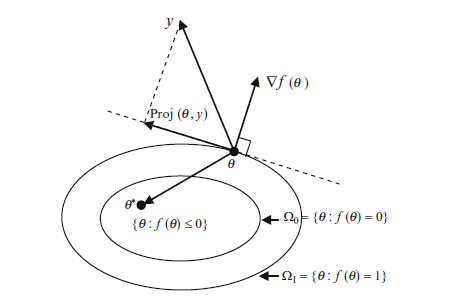
\includegraphics[width = 10cm]{figure/chap5/proj.png}
\bicaption[fig:chap5:F1]{射影算子示意图}{射影算子示意图}{Fig.}{Projection operator description}
\end{figure}
给出连续射影算子的示意形式:
\begin{equation}
\label{eq018}
Proj(\hat \theta, y) = \left\{\begin{matrix}
y- l f(\theta) y, & if [f( \theta) > 0   \quad and  \\
  &  (y\bigtriangledown f\left ( \theta \right ) >0 )]\\
y, & otherwise \\
\end{matrix}\right.\\
\end{equation}
其中,$l>0$是用来描述图中垂直与边界$\{ f(\theta) = \lambda,0 < \lambda < 1\}$的一个矢量的长度,矢量算子就成为从$\lambda =0$ 平滑到$\lambda =1 $的边界矢量的切线。

根据$l$的描述形式的不同,可以得到几种不同的矢量算子描述如下:

\begin{equation}
\label{eq018}
Proj(\hat \theta, y) = \left\{\begin{matrix}
y-   \frac{ \Gamma \bigtriangledown f(\theta) ( \bigtriangledown f(\theta)^T)}{\left \| \bigtriangledown f(\theta) \right \|_\Gamma ^T}  f(\theta) y, & if [f( \theta) > 0   \quad and  \\
  &  (y\bigtriangledown f\left ( \theta \right ) >0 )]\\
y, & otherwise\\
\end{matrix}\right.\\
\end{equation}
其中,$\Gamma$是任意的、正定的对称常数矩阵。

\begin{equation}
\label{eq018}
Proj(\hat \theta, y) = \left\{\begin{matrix}
y- \left \|   \bigtriangledown f\left ( \theta \right ) \right \| ^2 f(\theta) y, & if [f( \theta) > 0   \quad and  \\
  &  (y\bigtriangledown f\left ( \theta \right ) >0 )]\\
y, & otherwise \\
\end{matrix}\right.\\
\end{equation}

两种矢量算子的$l$的描述形式是不同的,本章中的分析主要采用其中一种进行推导分析,另一种算子可以采用相同方法进行处理。


\begin{lem}

令$f(\theta)$ 是从 $R^n$ 到$R$的一个连续可微的凸映射。基于上面给出的连续射影算子的公式,考虑

\begin{equation}
\dot \theta = Proj(\theta, y)
\end{equation}
其中,$\theta \in R^n$ 为系统状态,$y \in R^n$为时变的连续的分段矢量。那么对于所有的$t \geq 0$,对于集合0:

\begin{equation}
\Omega_0 = \{ \theta \in R^n | f(\theta) \leq 0\}
\end{equation}

对于集合0内的任意的初始条件为$\theta(0)=\theta_0$的系统轨迹 $\theta(t)$将维持在以下的集合内

\begin{equation}
\Omega_1 = \{ \theta \in R^n | f(\theta) \leq 1\}
\end{equation}

\begin{proof}

由于射影算子在$\theta$满足局部的Lipchitz条件\cite{lavretsky2013robust},同时系统外部输出$y(t)$在时间上是连续且分段的,因此解存在且唯一。

首先找到需要证明如下公式目标成立,即

\begin{equation}
\overbrace{[f(\theta_0) \leq 0 ]}^{\theta_0 \in \Omega_0} \Rightarrow \overbrace{[f(\theta(t)) \leq 1]}^{\theta(t)\in \Omega_1}, \forall t \geq 0
\end{equation}

首先给出射影算子为公式所列形式的时间导数:

\begin{equation}
\begin{aligned}
\dot{f}(\theta)&= (\bigtriangledown f(\theta))^T Proj(\theta,y)
         &= \left\{\begin{matrix}
\bigtriangledown f(\theta))^T y (1-f(\theta)), &  & if [
f(\theta) >0 \Lambda  y^T \bigtriangledown f >0 ] \\
\bigtriangledown f(\theta))^T y , &  & otherwise
\end{matrix}\right.
\end{aligned}
\end{equation}

因此,可以得出

\begin{equation}
\label{condi}
\begin{aligned}
\dot f(\theta) >0 ,&\mbox{如果} [0 < f(\theta) < 1 \quad \Lambda \quad   y^T\bigtriangledown f > 0]\\
\dot f(\theta) = 0, &\mbox{如果} [f(\theta) = 0 \quad \Lambda \quad  y^T\bigtriangledown f >0  ] \\
\dot f(\theta) \leq 0, &\mbox{如果} [f(\theta) \leq 0 \quad \Lambda \quad  y^T\bigtriangledown f \leq 0  ]
\end{aligned}
\end{equation}
公式\ref{condi}中,无论是哪种条件都可以保证 $\forall t \geq 0, f(\theta(t)\leq 1)$。

对于另外一种形式的射影算子,
\begin{equation}
\label{sheying}
\begin{aligned}
\dot f(\theta) &= \bigtriangledown f(\theta)^T \dot \theta (t)\\
  &=\bigtriangledown f(\theta)^T \left\{\begin{matrix}
  y - {\| \bigtriangledown f(\theta) \|}^2  f(\theta) y ,&  & if [
f(\theta) >0 \Lambda  y^T \bigtriangledown f >0 ]     \\
  y  ,&  & otherwise
\end{matrix}\right.\\
&= \bigtriangledown f(\theta)^T y (1- \|\bigtriangledown f(\theta)\|^2 f(\theta))
\end{aligned}
\end{equation}
其中,欧式平方范数满足$\| \bigtriangledown f \|^2 = (\bigtriangledown f)^T \bigtriangledown f$。在集合$\Omega_1$ 内, $\| \bigtriangledown f \|^2 \leq 1$。

公式\ref{sheying}中,无论是哪种条件都可以保证 $\forall t \geq 0, f(\theta(t)\leq 1)$。
\end{proof}
\end{lem}

引理5.5是自适应控制器的设计是非常重要的结果,对于前面的带有有界干扰的模型参考自适应控制,可以得到误差动态的李雅普诺夫函数:
\begin{equation}
\begin{array}{l}
\begin{split}
 \dot V =  - {e^T}Qe + 2e^{T}P\varepsilon &+ 2tr\left( {\Delta K_x^T\left[ {\Gamma _x^{ - 1}{{\dot {\hat K}}_x} + x{e^T}PB} \right]\Lambda } \right) \\
 &+  2tr\left( {\Delta K_r^T\left[ {\Gamma _r^{ - 1}{{\dot {\hat K}}_r} + x{e^T}PB} \right]\Lambda } \right) \\
 &+ 2tr\left( {\Delta {\Theta ^T}\left[ {\Gamma _\Theta ^{ - 1}\dot {\hat \Theta}  - \Phi \left( x \right){e^T}PB} \right]\Lambda } \right) \\
 \end{split}
 \end{array}
\end{equation}
为了保证系统稳定,就要确保李雅普诺夫函数为半负定,那么

\begin{equation}
\begin{aligned}
tr\left( {{\underbrace {\Delta K_x}_{\hat K_x - K_x}}^T\left[ {\Gamma _x^{ - 1}{\underbrace{\dot{\hat K}_x}_{Proj(\hat \theta, \Gamma _x Y)}} + \underbrace {x{e^T}PB}_{Y}} \right]\Lambda } \right) \\
= \sum_{j = 1}^{m}\underbrace{(\hat {K}_x - {K}_x)_j^T(\Gamma_x^{-1} Proj(\hat
x,\Gamma_x Y_j)-Y_j}_{\leq 0})\underbrace{\lambda_j}_{\geq 0} \leq 0
\end{aligned}
\end{equation}

因此可以定义基于射影理论的自适应律如下:

\begin{equation}
\dot {\hat{\Theta}} = Proj(\hat{\Theta},\Gamma_x x e^T PB)
\end{equation}

参考引理5.5,可以确定自适应律$K_{x}$具有一致有界性。关于$K_r$和$\Theta$ 的一致有界性也可以采用类似的方法证明。

本质上,射影算子确保了$\hat K_x$ 的第 $j$ 列不超过其预定的界限$\Theta_j^{max}$。因此射影算子给李雅普夫函数带了负半定性。
\begin{equation}
\begin{aligned}
\dot V(e,\Delta K_x) &\leq - e^T Q e + 2 e^T P \varepsilon \\
&\leq -\lambda_{min}(Q) \|e \|^2 + 2  \|e \| \lambda_{max}(P) \varepsilon_{max}\\
&=-\lambda_{min}(Q) \|e \|(\|e \| - 2\frac{\lambda_{max}(P)\varepsilon_{max}}{\lambda_{min}(Q)})
\end{aligned}
\end{equation}

因此,在紧集中,

\begin{equation}
\Omega = \{(e,\Delta K_x) \in R^n \times R^{N \times m}: \|e \| \} \leq 2\frac{\lambda_{max}(P) \varepsilon_{max}}{\lambda_{min}(Q)} \quad \Lambda \quad  \| \bigtriangleup K_x \|_F \leq \bigtriangleup {K_x}_{max}
\end{equation}

根据引理5.5,在紧集外部,可以有
\begin{equation}
\dot  V (e, \bigtriangleup K_x) < 0
\end{equation}
其中,
\begin{equation}
\begin{aligned}
&\bigtriangleup {K_x}_{max} \\
&= 2\underbrace{(({K_x^{max}}_1) ,..., {K_x^{max}}_{m}))}_{{K_x}_{max}}\\
& = 2 {K_x}_{max}
\end{aligned}
\end{equation}

因此,射影算子改造的增益$K_x$具有边界,不会无限制的,克服了前面的参数漂移问题,故可以证明射影算子改造的自适应控制律可以以有界误差跟任意外部有界指令。



\subsubsection{基于射影算子的MRAC }

考虑到水下航行器的模型是一个动态系统,包含多输入和多输出,具有不确定性、有界干扰和未建模动力学,动态系统可以定义如下:

\begin{equation}
\label{eq012}
\begin{array}{l}
\dot{\bm{x}}(t) = \bm{A} \bm{x}(t)+ \bm{B} \bm{\Lambda}u + \bm{\xi} (t)\\
\bm{y}(t) = \bm{C}\bm{x} (t)
\end{array}
\end{equation}
其中$\bm{\xi(t)}$是一个随时间变化的有界扰动,因此可以得到$\left \| \bm{\xi}(t) \right \| \leq \bm{\xi}_{max}$。 $\Theta ^{T}\Phi (\bm{x})$表示动态系统的非线性项。 $\bm{A}$是动态系统的状态转换矩阵。 $\bm{B}$是动态系统的输入矩阵,$\bm{C}_{ref}$是输出矩阵。$\bm{\Lambda} > 0$是用来表示控制效率的对角矩阵。

为了设计受到有界扰动的水下机器人的状态反馈鲁棒射影自适应控制器,可以定义参考模型:

\begin{equation}
\label{eq013}
\begin{array}{l}
\bm{\dot x}_{ref} (t)= \bm{A}_{ref}\bm{x}_{ref}(t)+\bm{B}_{ref}\bm{r}(t) \\
\bm{y}_{ref}(t) = \bm{C}_{ref}\bm{x}_{ref}(t)
\end{array}
\end{equation}
其中,$\bm{A}_{ref}$ 表示参考模型的状态传递矩阵,且是$Hurwitz$阵;$\bm{B}_{ref}$是参考模型的输入矩阵。公式中的参数满足如下关系,
$\bm{B}_{ref} = \bm{B}k_g$,在该式中,$k_g = {}\frac{-1}{\bm{C}^T \bm{A}_m^{-1} \bm{B}}$,是用来求出消除稳态追踪误差。此外,$\bm{C}_{ref} = \bm{C}$.

根据等式\ref{eq012}和\ref {eq013},可以给出鲁棒模型参考自适应的控制律如下:

\begin{equation}
\label{eq014-5}
u = \hat{\bm{K}}_x ^{T}(t)\bm{x}(t) + \hat{\bm{K}}_r ^{T}(t)\bm{r}(t)
\end{equation}
其中,$\hat{\bm{K}}_x$, $\hat{\bm{K}}_r$分别是与状态和输入有关的更新律,并通过迭代估计获得相对应的参数。

将公式\ref{eq014-5}代入公式\ref{eq012}中,动态系统的状态参考模型变为

\begin{equation}
\label{eq015}
\bm{\dot x}(t)=(\bm{A}+\bm{B}\bm{\Lambda}{\hat{\bm{K}}_x}^T)\bm{x}
+ \bm{B} \bm{\Lambda}\hat{\bm{K}}_r ^{T}(t)\bm{r}(t)
\end{equation}

定义状态跟踪误差如下:
\begin{equation}
\bm{e}(t) = \bm{x}(t) - \bm{x_{ref}}(t)
\end{equation}

将公式\ref{eq013} 和公式\ref{eq015}分别代入状态跟踪误差中并求导,则可以获得跟踪误差动态如下:

\begin{equation}
\label{eq016}
\dot{\bm{e}}(t) = \bm{A}_{ref}\bm{e}(t)-\bm{B}\Lambda (\Delta \hat{\bm{K}}_x ^{T}(t) \bm{x}(t) + \Delta \hat{\bm{K}}_r ^{T}(t)\bm{r}(t)) + \bm{\xi}_(t)
\end{equation}
其中, $\Delta {\bm{K}}_x = \hat{\bm{K}}_x - {\bm{K}}_x$,  $\Delta {\bm{K}}_r = \hat{\bm{K}}_r - {\bm{K}}_r$ 分别是参数的估计误差。控制器参数 $\hat{\bm{K}}_x$ 与 $\hat{\bm{K}}_r$ 可以使用自适应律进行更新估计。

在存在有界干扰的情况下,受噪声影响时控制器不够稳定。然而,基于投影算子的自适应算子控制律可以实现自适应参数的快速自适应和均匀一致有界性。它还可以保持水下机器人系统以及相应的误差动态的闭环稳定性。 自适应更新法则可以被重写:

\begin{equation}
\label{eq017}
\begin{array}{l}
{\dot{\hat{\bm K}}_x (t)}=Proj(\hat{\bm K}_x(t),-\bm{\Gamma}_x \bm{x}(t) {\bm e}(t)\bm{PB}sgn(\bm \Lambda)) \\
{\dot{\hat{\bm K}}_r (t)}=Proj(\hat{\bm K}_r(t),-\bm{\Gamma}_r \bm{r}(t) {\bm e}(t)\bm{PB}sgn(\bm \Lambda))
\end{array}
\end{equation}
其中,
\begin{equation}
\label{eq018}
Proj(\hat \theta, y) = \left\{\begin{matrix}
y- \left \|   \bigtriangledown f\left ( \theta \right ) \right \| ^2 f(\theta) y & if [f( \theta) > 0   \quad and  \\
  &  (y\bigtriangledown f\left ( \theta \right ) >0 )]\\
y & otherwise \\
\end{matrix}\right.\\
\end{equation}
并且,$f(\theta)$是凸函数,具体定义如下

\begin{equation}
\label{eq019}
\begin{array}{l}
f(\theta)={}\frac{\left ( 1+ \epsilon  \right )\left \| \theta  \right \|^2 - \theta _{max}^2}{\epsilon \theta_{max}^2}\\
\\
\bigtriangledown f(\theta)={}\frac{2 \theta(1+\epsilon )}{\epsilon \theta _{max}^2}
\end{array}
\end{equation}
其中,$\epsilon$是投影公差,并且$\theta_{max}$是参数边界。 需注意,公式\ref {eq018}和公式\ref {eq019}中的$\theta$ 不是之前定义的水下机器人的俯仰角,它只是一个参数符号变量。 $P$可以通过求解Lyapunov方程得出,

\begin{equation}
\bm{A_m}^T \bm{P} + \bm{P} \bm{A_m} = -\bm{Q}
\end{equation}
其中,$\bm{Q}$ 是任意的正定矩阵。


\subsection{$L_{1}$自适应控制 }


在本节中,针对具有不确定性和输入饱和的系统,引入具有快速自适应律与鲁棒性的$L_1$自适应控制方法。模型参考自适应控制架构的控制方法是采用更新自适应律来跟踪参考模型的,但是参考模型的所能够表征动态系统是有限的,此外,鲁棒模型参考自适应控制的框架下,实现的自适应更新是以牺牲响应速度换来的自适应,这对于剧烈变换的未知环境是不利的。水下机器人的环境具有未知、难预测的特性,因此要实现水下机器人在深海的生存能力还应关注自适应的响应速度问题。此外,在自适应控制中,自适应更新会给机器人的控制带来动态的干扰,而水下机器人尤其是鱼雷型机器人的各个自由度之间是严重耦合,这样就需要水下机器人给系统带来尽量少的瞬态响应。$L_1$自适应控制不仅采用射影算子修正的自适应律还通过解耦适应率和鲁棒性来保证了控制器的瞬态响应,以及采用合适的滤波器降低高频震荡信号的影响\cite{maalouf2013contribution}。

在动态系统中需要考虑不确定性的问题,$L_1$自适应控制中采用状态模型如下:
\begin{equation}
\begin{array}{l}
 \dot x = Ax + B(\omega u(t) + f(t,x(t))) \\
 y = {C^T}x(t) \\
 \end{array}
\end{equation}
其中,$x(0)= x_0$; $ x_0 $是有界集的状态初始条件; $ A $是系统状态变量; $y$是系统测量的输出; $B$和$C$是为驱动器和观察定义的矢量; $u$是用于控制系统的输入; $\omega$是一个未知的有界参数,表示不确定命令的效率; $f(t,x(t))$是一个不明确定义的非线性项,表示未建模的动态。

这个控制器的目的是在存在未知的$A$ 和 $f(t,x(t))$的情况下追踪所需的 $r(t)$。 考虑$Hurwitz$矩阵$A_{ref}$来表达系统矩阵,并重写动态系统中的非线性项如下:
\begin{equation}
f(t,x(t)) = {A_2}{x_2} + \theta (t){\left\| {x(t)} \right\|_{L\infty }} + \sigma (t)
\end{equation}
其中, $\theta(t)$ 、 $\sigma(t)$ 是未知且时变的参数。

在存在不确定性时, 当控制器根据如下所述的参考系统模型跟踪控制输入信号时,可以获得期望的追踪性能:

\begin{equation}
\begin{array}{l}
 \dot{\hat{x}} = {A_m}\hat x(t) + {B}(\hat \omega (t)u(t) + \hat \theta (t){\left\| {x(t)} \right\|_{L \propto }} + \hat \sigma (t)) \\
 \hat y = {C^T}\hat x(t) \\
 \end{array}
 \end{equation}
这里,$\hat \omega (t)$, $\hat \theta (t)$ 以及 $\hat \sigma (t)$ 是在每次迭代中自适应律获得的估计参数。

然后使用实际系统的测量状态和估计值形成模型的误差信号。
\begin{equation}
\tilde x(t) = \hat x(t) - x(t)
\end{equation}
因此,误差可以用于计算自适应律来调整参数,其中采用投影方法来确保均匀一致有界性。此外,投影算子可以保持闭环系统的稳定性并实现快速适应。自适应律的计算使用公式\ref{eq017}中所示的等式来完成:

\begin{equation}
\begin{array}{l}
 \dot {\hat {\theta }}(t) = {{\boldsymbol{\Gamma }}_\theta } {\rm{Proj}}(\hat \theta (t), - {{\tilde x}^T}(t){\left\| {x(t)} \right\|_{{\rm{L}}\infty }}PB) \\
 \dot {\hat {\sigma }}(t) = {{\boldsymbol{\Gamma }}_\sigma } {\rm{Proj}}(\hat \sigma (t), - {{\tilde x}^T}(t)PB) \\
 \dot {\hat {\omega }}(t) = {{\boldsymbol{\Gamma }}_\omega } {\rm{Proj}}(\hat \omega (t), - {{\tilde x}^T}(t)u(t)PB) \\
 \hat {\theta } (0)= {{\hat \theta }_0} \\
 \hat {\sigma } (0)= {{\hat \sigma }_0} \\
 \hat {\omega } (0)= {{\hat \omega }_0} \\
 \end{array}
 \end{equation}
其中,$\boldsymbol{\Gamma} \in {\mathbf{R}}^{ + }$ 是自适应增益。当设定任意对称矩阵 $Q=Q^{T}>0$,对称的正定对角矩阵 $P$ 是李雅普诺夫方程的解 $A_m^TP + P{A_m} =  - Q$ 。

然后在控制输入阶段,通过在频域添加低通滤波器获得的$L_1$自适应的控制信号:

\begin{equation}
\begin{array}{l}
 {u_a}(s) =  - kD(s)(\hat \mu (s) - {k_g}r(s)) \\
 \hat \mu (s) = \ell \left\{ {\hat \mu } \right\}{\rm{ = }}\ell \left\{ {\hat \omega (t)u(t) + \hat \theta (t){{\left\| {x(t)} \right\|}_{{\rm{L}}\infty }} + \hat \sigma (t)} \right\} \\
 \end{array}
 \label{eq:chap5:59}
\end{equation}
这里,$D(s)$ 是一个用来过滤高频信号的传递函数。$k$ 是反馈增益,$k_g=-(CA_{m}^{-1}B_m)^{-1}$ 是用来处理输入参考指令 $r(t)$ 的增益。


\subsection{水下机器人俯仰控制实验 }

为了验证本章提出的控制方法,使用REMUS AUV进行控制仿真的实验。如第四章的介绍,俯仰自由度的模型是被简化过的,且在本节中是要控制的自由度。时变参考指令被输入到控制系统里,用来测试控制器追踪性能。这些测试是使用不同的动态模型系统进行的,并且对比了不同的控制器的性能。

仿真实验是在MATLAB/Simulink中进行测试的,在所有的测试中,初始位置与姿态均为零,水下机器人被控制着以追踪时变姿态指令。在实际REMUS实验中,无论采用哪种控制器,横滚自由度在开始的20s内都出现振动,这种行为是因为REMUS机器人的横滚自由度是不可控的,这种振动无法使用控制的方式进行补偿。首先基于不同潜水控制系统模型的动态系统模型,分别设计不同的鲁棒自适应控制器方法进行仿真测试。在仿真中使用两种不同的运载器深度模式的动态系统。 一个是简化的基于线性的深潜模型动态系统,另一个是从实验中提取的REMUS AUV的6自由度非线性动力学模型\cite{prestero2001development,prestero2001verification}。

本节首先介绍线性系统和非线性模型系统的动力学模型与参数。线性俯仰模型系统的相关参数给出如下:$ A= [-0.8200,-0.6900; 1.0000,0]$,$B = [ - 4.1600; 0]$ 。鲁棒自适应控制器是基于状态方程的形式设计的,因此可以基于线性模型系统给出参考模型的相关参数:$ A_ {ref} = [ - 1.0900,-0.5200; 1.0000,0]$,$ B_ {ref} = [0.5200;0]$。无论是鲁棒模型参考自适应控制,还是$L_1$自适应控制两种方法的参考模型都是相同的,但是鲁棒模型参考自适应控制与$L_1$自适应的控制器的具体参数因系统而定义。鲁棒模型参考自适应控制的相应控制器参数给出如下:$K_x$ 和 $K_r$ 的 $\theta_ {max}$ 分别为 $300$ 和 $100$。 对于每个自适应更新律,投影公差 $\epsilon$ 为 $0.3$,对于每个自适应更新律 $\bm{\Gamma}$ 为 $10$。 在Lyapunov方程中 $\bm {Q} $ 是 $[20,0; 0,200]$。


本节在对控制器的性能进行研究时,主要考虑了水下机器人系统所可能承受的如下几种情况:1. 噪声,主要包括驱动器、传感器测量以及期望跟踪指令自带的噪声;2. 干扰,主要是不可以预测的干扰,该干扰和控制信号处于同一个数量级,影响性不可忽视;3. REMUS水下机器人自身的系统动力学特点,主要包括耦合扰动和非线性。

噪声是高斯白噪声,采用信噪比公式可以很好的观测不同SNR值下的控制器响应,本节中具体噪声参数如下:输入指令噪声(噪声功率:2.89e-6),状态测量噪声(噪声功率:2.36e-6)。水下机器人系统在水里运动受到的干扰是采用脉冲信号来分析,干扰与时间的关系如图\ref{fig:chap5:F4},且干扰是加载到俯仰角上的。

\begin{figure}[!htp]
\label{fig:chap5:F4}
\centering
\subfigure{
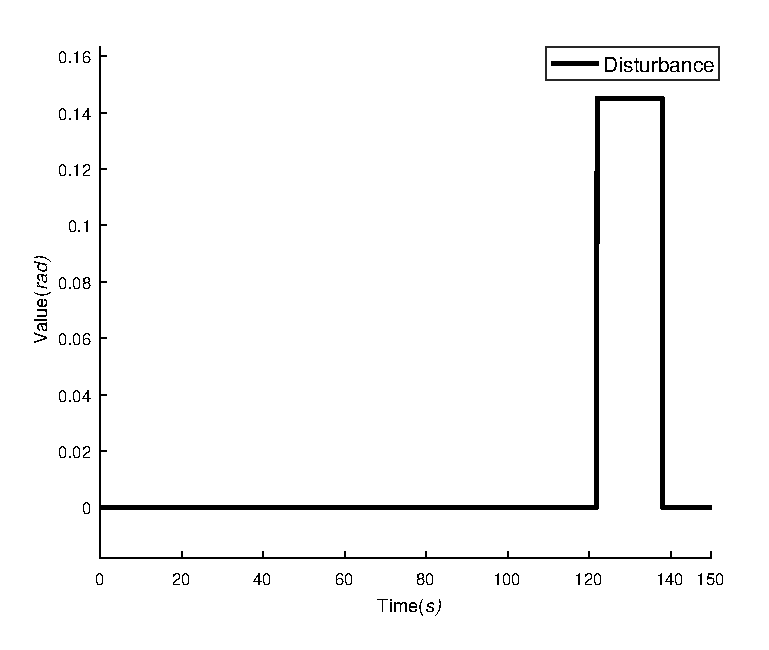
\includegraphics[width = 9cm]{figure/chap5/6dof/L1AC/disturbance.pdf}
}
\bicaption[fig:chap5:F4]{俯仰角的干扰信号}{俯仰角的干扰信号}{Fig.}{Disturbance in the pitch angle $\theta_a$}
\end{figure}


\begin{figure*}[htp]
\centering
\begin{minipage}{0.8\linewidth}
  \centerline{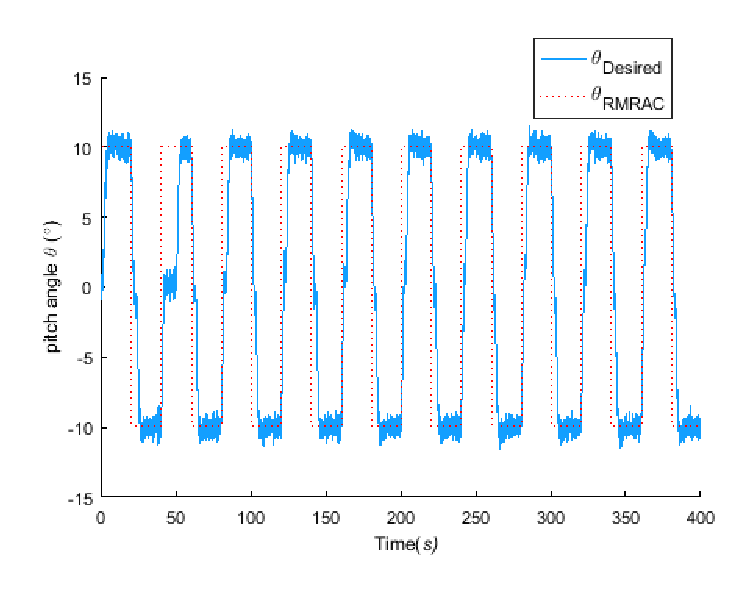
\includegraphics[width=13.0cm,height = 8cm]{figure/chap5/linear/RMRAC/RMRAC_x.pdf}}
  \centerline{(a) }
\end{minipage}
\vfill
\begin{minipage}{0.48\linewidth}
  \centerline{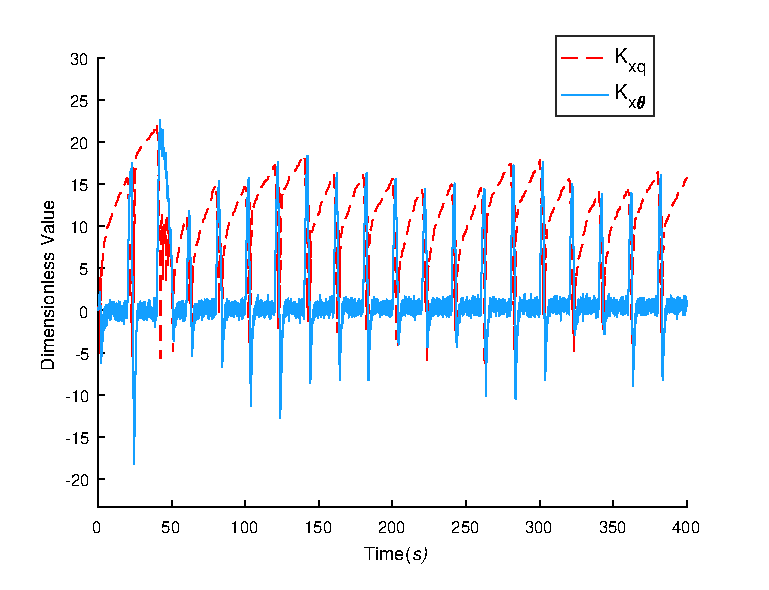
\includegraphics[width=8.0cm,height = 6cm]{figure/chap5/linear/RMRAC/K_x.pdf}}
  \centerline{(b) }
\end{minipage}
\hfill
\begin{minipage}{0.48\linewidth}
  \centerline{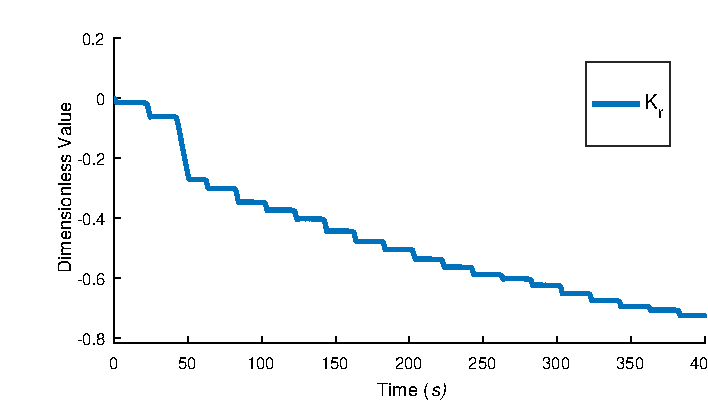
\includegraphics[width=7.0cm,height = 6cm]{figure/chap5/linear/RMRAC/K_r.pdf}}
  \centerline{(c) }
\end{minipage}
\label{fig:chap5:F2}
\bicaption[fig:chap5:F2]{存在驱动噪声和测量噪声时线性动态系统的鲁棒模型参考自适应控制追踪脉冲输入指令}{存在驱动噪声和测量噪声时线性动态系统的鲁棒模型参考自适应控制追踪脉冲输入指令}{Fig.}{ Robust model reference adaptive control of linear dynamic systems for tracking pulse input set-points in the presence of measurement and actuator noise}
\end{figure*}


\begin{figure*}[!htp]
\centering
\begin{minipage}{0.8\linewidth}
  \centerline{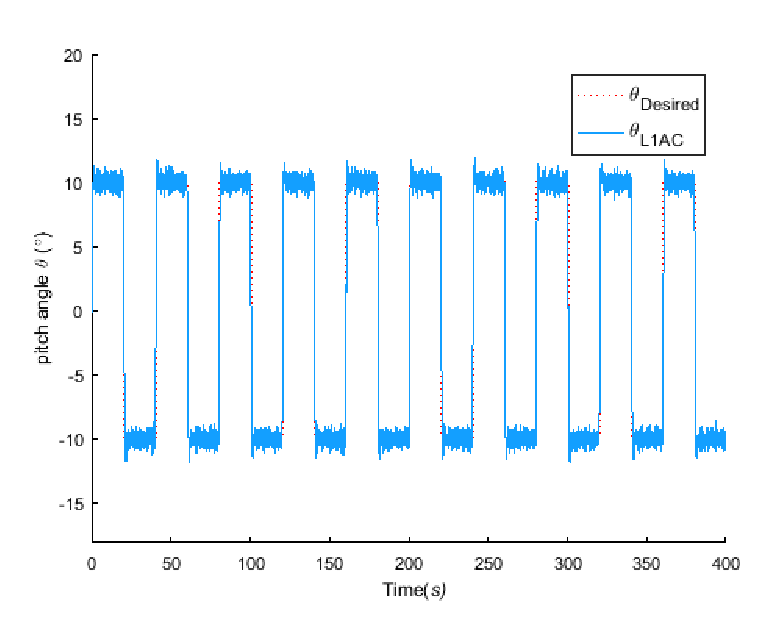
\includegraphics[width=13.0cm,height = 7cm]{figure/chap5/linear/L1AC/L1AC_x.pdf}}
  \centerline{(a) }
\end{minipage}
\vfill
\begin{minipage}{0.48\linewidth}
  \centerline{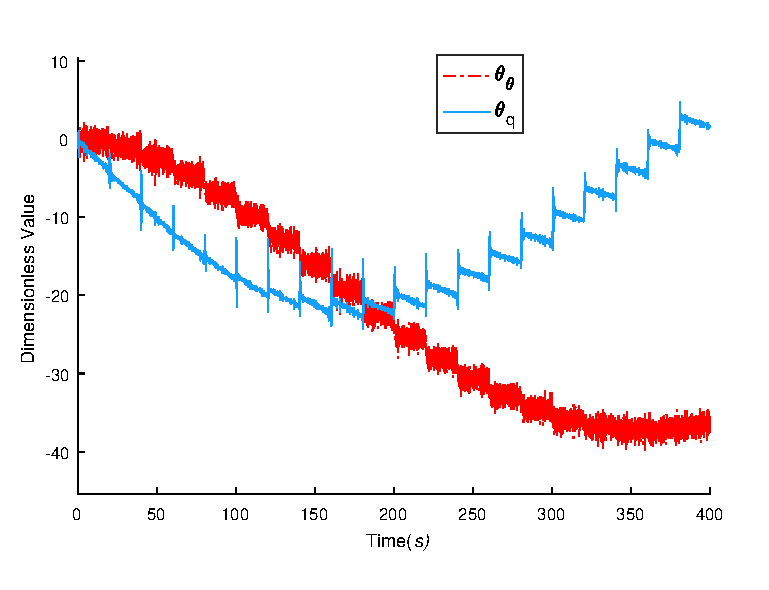
\includegraphics[width=7.0cm,height = 4.5cm]{figure/chap5/linear/L1AC/Theta.pdf}}
  \centerline{(b) }
\end{minipage}
\hfill
\begin{minipage}{0.48\linewidth}
  \centerline{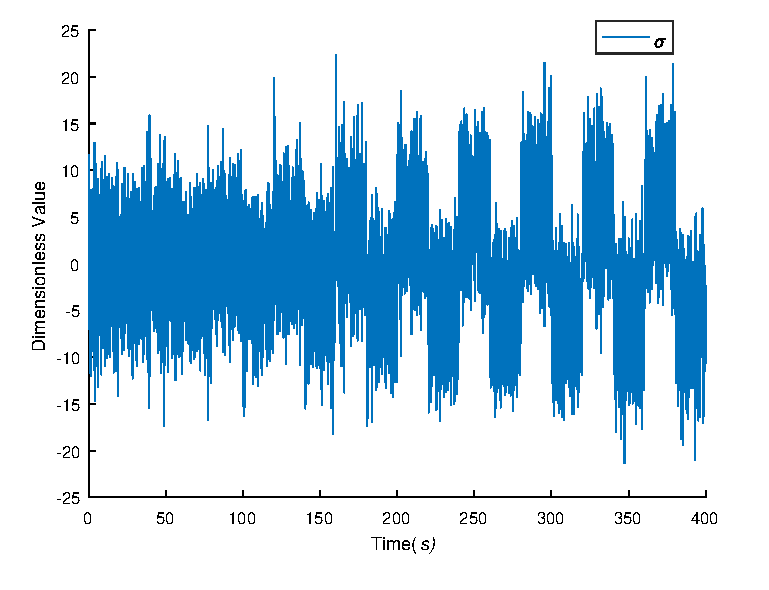
\includegraphics[width=7.0cm,height = 5cm]{figure/chap5/linear/L1AC/Sigma.pdf}}
  \centerline{(c) }
\end{minipage}
\vfill
\begin{minipage}{0.48\linewidth}
  \centerline{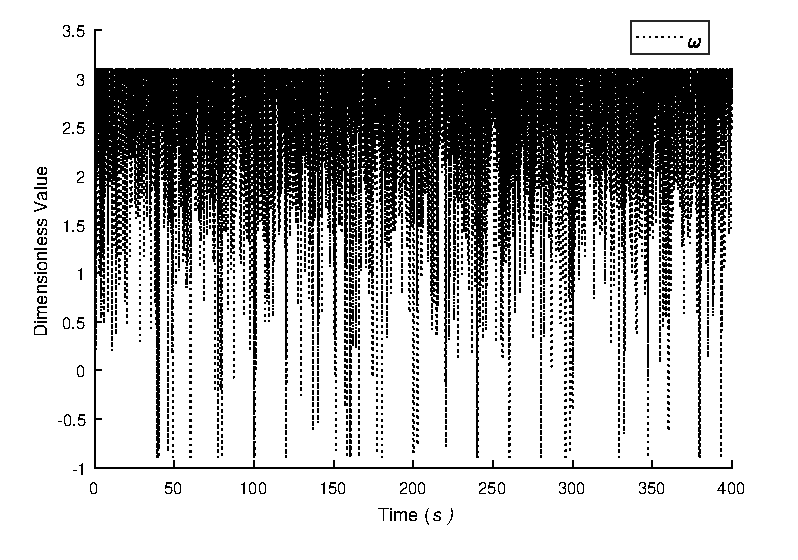
\includegraphics[width=7.0cm,height = 5cm]{figure/chap5/linear/L1AC/omega.pdf}}
  \centerline{(d) }
\end{minipage}
\label{fig:chap5:F3}
\bicaption[fig:chap5:F3]{存在驱动噪声和测量噪声时线性动态系统的 \texorpdfstring {$L_1$}{}{自适应控制} } {存在驱动噪声和测量噪声时线性动态系统的 \texorpdfstring {$L_1$}{}{自适应控制} } {Fig.}{ \texorpdfstring {$L_1$}{} {adaptive control of linear dynamic systems for tracking pulse input set-points in the presence of measurement and actuator noise} }
\end{figure*}

\subsubsection{线性系统模型俯仰控制实验 }

给定脉冲输入指令,并考虑驱动器输入和状态测量存在噪声的情况,使用鲁棒模型参考自适应控制来追踪期望指令,如图\ref{fig:chap5:F2}。图\ref{fig:chap5:F2}中a图包括俯仰角度的状态响应与期望指令的对比,图\ref{fig:chap5:F2}中b和c图分别给出了鲁棒自适应控制的自适应更新参考$K_x$,$K_r$的响应曲线。可以发现图\ref{fig:chap5:F2}中a图的期望角度跟踪情况是不断优化和更新,这是因为自适应参数不断进化以缩小误差,到最后的一个50s周期时候,控制效果已经比第一个与第二个周期改善很多。虽然存在输入噪声和测量噪声,鲁棒自适应控制器也能够进行正常工作,这说明基于投影算子的自适应更新律可以很好地解决有界噪声扰动问题。

将脉冲输入指令输入到$L_1$自适应控制器中,并考虑驱动器噪声和测量噪声,可以获得控制性能追踪影响曲线与$L_1$自适应控制器的自适应参数曲线如图\ref{fig:chap5:F3}。相比于鲁棒自适应控制自适应更新计算速率慢,$L_1$自适应控制可以让控制器很好地跟踪期望指令,并且响应的速率更快,很难看出自适应的更新过程。因为$L_1$自适应控制的自适应更新律是基于投影算子的,因此$L_1$自适应控制也能够很好地应对有界噪声干扰的问题。对比鲁棒自适应控制和$L_1$自适应控制方法的俯仰角度跟踪过程,前者的自适应更新具有很长的时间区间,而后者的自适应过程很难被察觉出来。

简化的线性动态系统可以用来初步验证所提出的控制方法的可行性,但是要用于水下机器人的复杂多自由度系统的控制就需要更深入的讨论。

\subsubsection{6自由度非线性系统模型 俯仰控制实验 }

用于自适应控制的模型一般是对非线性模型进行简化获得。然而,航行器控制器的性能很容易受到驱动器的非线性和模型中的不确定性的影响。使用本文中提出的鲁棒自适应控制和$L_1$自适应控制用于REMUS的6自由度非线性模型系统的俯仰自由度的控制,并使用MATLAB/Simulink进行仿真,以对控制器的性能进行充分验证。

在存在驱动器噪声、测量噪声、干扰的情况下,采用鲁棒自适应控制和$L_1$自适应控制方法用于REMUS水下机器人的非线性模型的俯仰自由度的控制。REMUS的6自由度模型系统具有高度非线性,并且由于浮力大于重力,这使得REMUS系统成为了一个静不平衡非线性动态系统。俯仰自由度的控制中包含了不确定性和有界干扰,这可以很好地验证自适应控制器的性能。

\begin{figure}[!htp]
\centering
\begin{minipage}{0.9\linewidth}
  \centerline{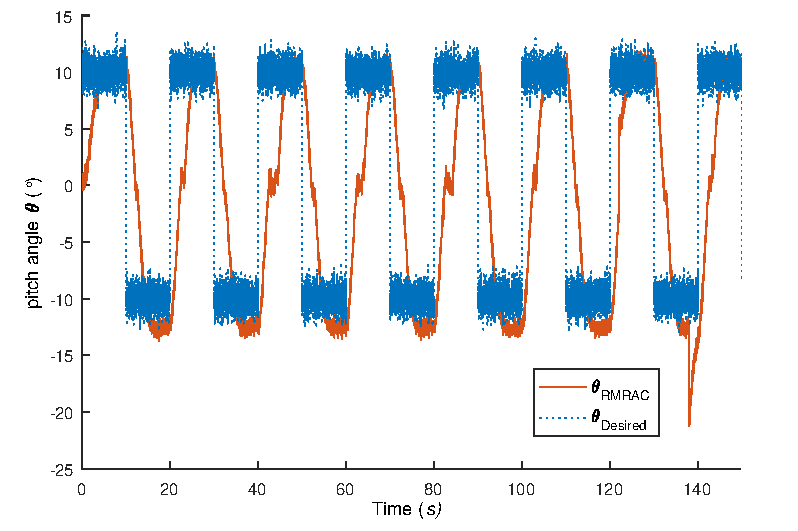
\includegraphics[width=12.0cm,height = 7cm]{figure/chap5/6dof/RMRAC/RMRA_x_pulse.pdf}}
  \centerline{(a) }
\end{minipage}
\vfill
\begin{minipage}{0.48\linewidth}
  \centerline{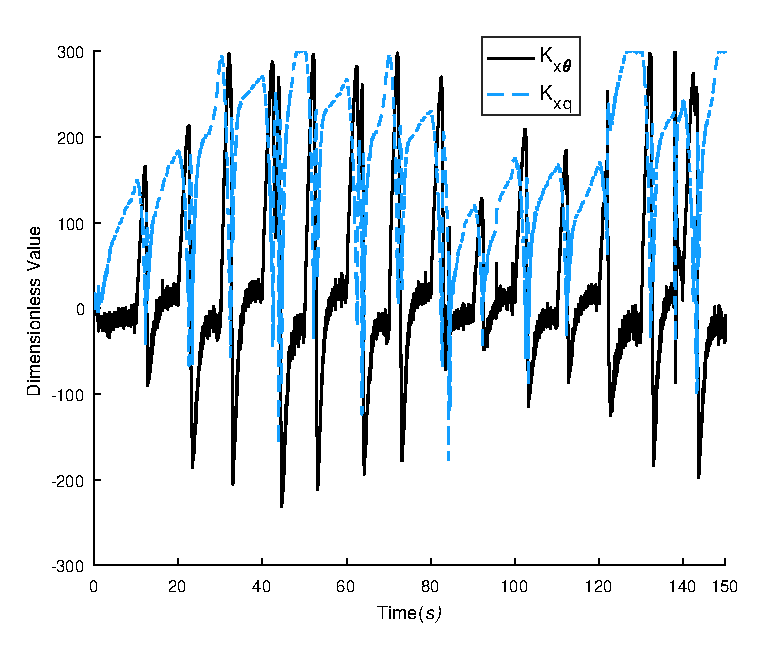
\includegraphics[width=7.0cm,height = 5cm]{figure/chap5/6dof/RMRAC/K_x.pdf}}
  \centerline{(b) }
\end{minipage}
\hfill
\begin{minipage}{0.48\linewidth}
  \centerline{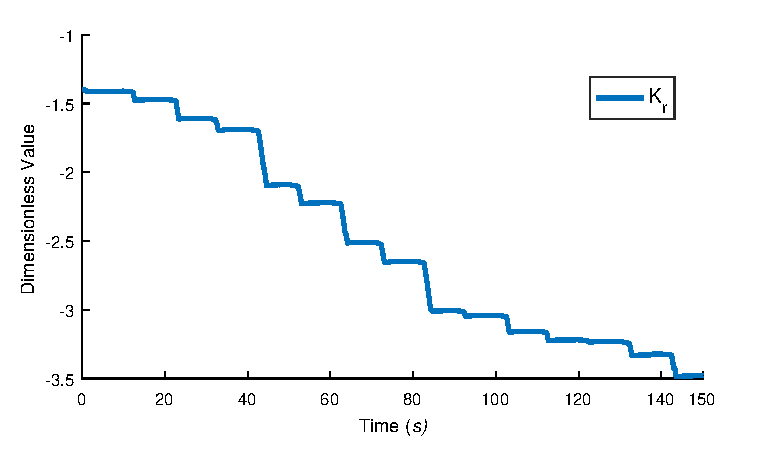
\includegraphics[width=7.0cm,height = 5cm]{figure/chap5/6dof/RMRAC/K_r.pdf}}
  \centerline{(c) }
\end{minipage}
\label{fig:chap5:F5}
\bicaption[fig:chap5:F5]{存在驱动噪声、测量噪声和干扰时6自由度非线线性动态系统的鲁棒模型参考自适应控制追踪脉冲输入指令}{存在驱动噪声、测量噪声和干扰时6自由度非线性动态系统的鲁棒模型参考自适应控制追踪脉冲输入指令}{Fig.}{ Robust model reference adaptive control of the 6 DOF nonlinear dynamic systems for tracking pulse input set-points in the presence of measurement actuator noise and disturbance}
\end{figure}

对比图\ref{fig:chap5:F5}和图\ref{fig:chap5:F7}可以发现,鲁棒自适应控制的自适应进化过程相比于$L_1$自适应控制方法更加缓慢,两种控制方法都能够应对驱动器、测量单元以及输入指令的有界干扰。

文中为了更好的显示$L_1$自适应控制跟踪期望指令的响应曲线,$L_1$控制的对比期望指令是理想的,但实际控制器接收的输入指令是带有噪声的。由于水下机器人具有正浮性,且REMUS机器人是主要依靠舵片控制俯仰角度与深度,因此,俯仰自由度的控制的状态响应与期望指令之间存在稳态误差,且$L_1$自适应克服稳态误差的效果更好。


此外,鲁棒自适应控制器和$L_1$自适应控制器的应对未建模扰动的性能也进行了对比,鲁棒模型参考自适应控制的俯仰角度受到的干扰后的俯仰角波动更剧烈,这也进一步验证了$L_1$自适应控制方法的鲁棒性。

REMUS试下机器人模型系统是高度耦合且非线性的,各个状态间的互相扰动情况也应当注意,可以发现鲁棒自适应控制器由于自适应律更新慢,俯仰角速率更小,这使得横滚自由度内的动态响应也更加缓慢,如图\ref{fig:chap5:F6}和图\ref{fig:chap5:F8}。

为了进一步对比鲁棒自适应控制和$L_1$自适应控制方法的效果,正弦输入指令被输入到自适应控制器。图\ref{fig:chap5:F9}给出了存在驱动噪声、测量单元噪声、输入指令噪声以及干扰时的REMUS水下机器人模型的俯仰角度进行鲁棒自适应控制和$L_1$自适应控制的角度响应结果。可以发现,$L_1$自适应控制的自适应律计算速度更快,且应对干扰的能力更强。
\begin{figure}[htp]
\centering
\begin{minipage}{0.48\linewidth}
  \centerline{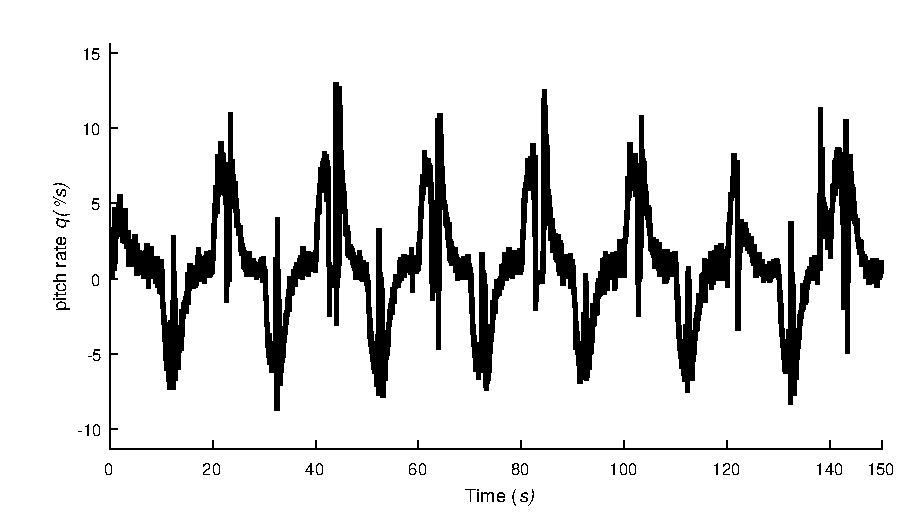
\includegraphics[width=8.0cm,height = 6cm]{figure/chap5/6dof/RMRAC/pitch_rate_q.pdf}}
  \centerline{(a) }
\end{minipage}
\hfill
\begin{minipage}{0.48\linewidth}
  \centerline{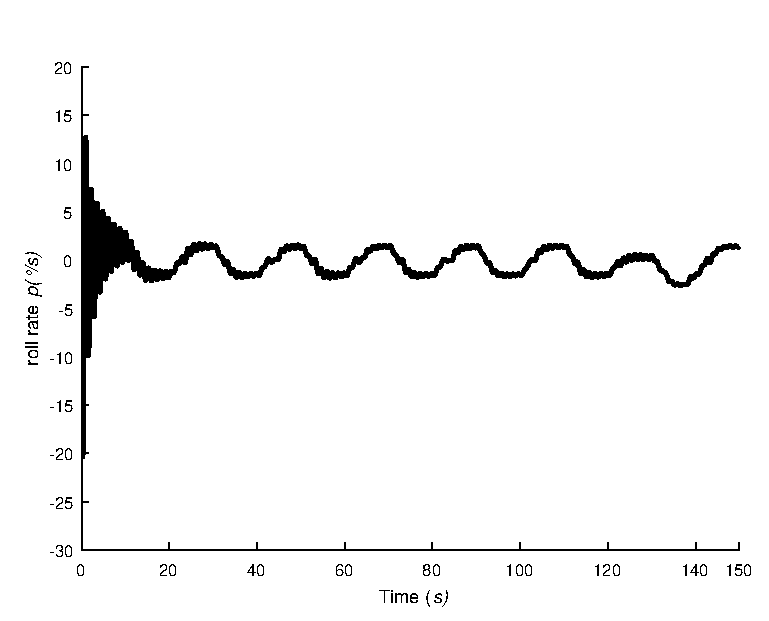
\includegraphics[width=8.0cm,height = 6cm]{figure/chap5/6dof/RMRAC/roll_rate_p.pdf}}
  \centerline{(b) }
\end{minipage}
\label{fig:chap5:F6}
\bicaption[fig:chap5:F6]{6自由度非线性动态系统的鲁棒模型参考自适应控制追踪脉冲输入指令的俯仰与横滚速率响应}{6自由度非线性动态系统的鲁棒模型参考自适应控制追踪脉冲输入指令的俯仰与横滚速率响应}{Fig.}{ Pitch and roll rate response of the robust model reference adaptive control of 6 DOF nonlinear vehicle when tracking pulse input set-points}
\end{figure}

\begin{figure}[htp]
\centering
\begin{minipage}{0.9\linewidth}
  \centerline{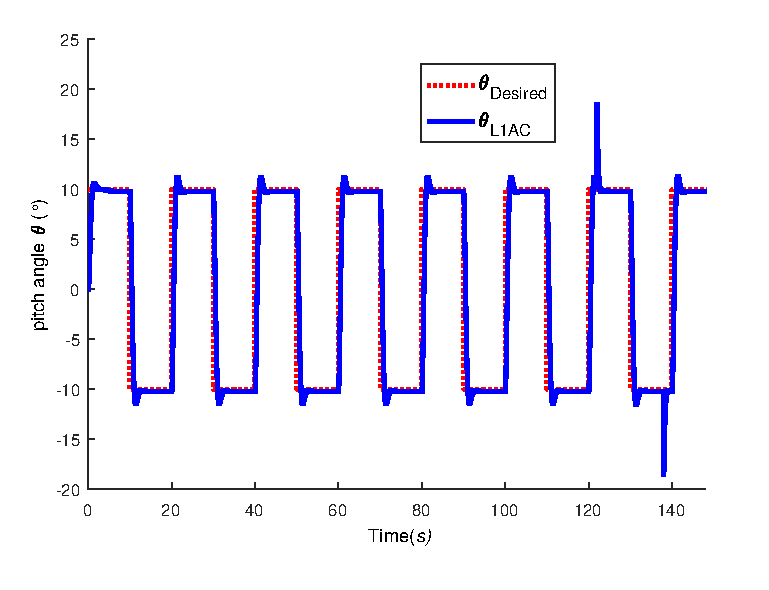
\includegraphics[width=12.0cm,height = 7cm]{figure/chap5/6dof/L1AC/L1AC_x_pulse.pdf}}
  \centerline{(a) }
\end{minipage}
\vfill
\begin{minipage}{0.48\linewidth}
  \centerline{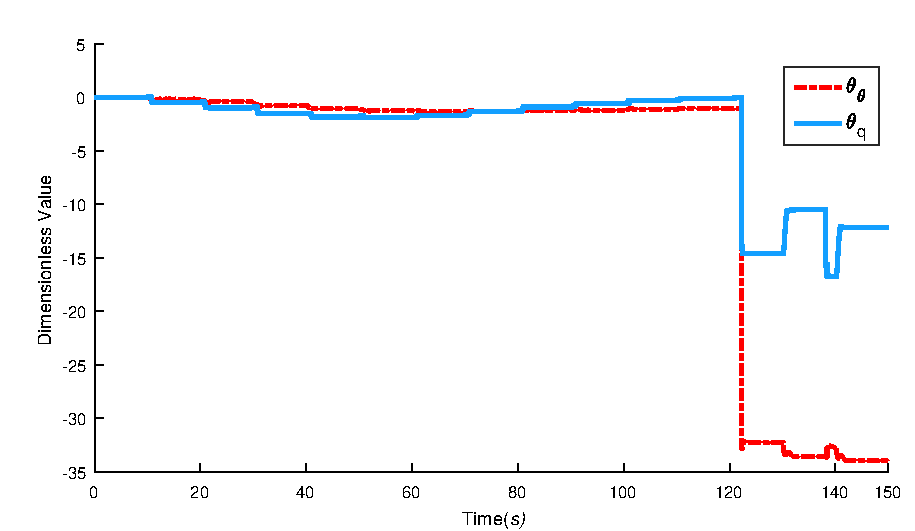
\includegraphics[width=7.0cm,height = 5cm]{figure/chap5/6dof/L1AC/Theta.pdf}}
  \centerline{(b) }
\end{minipage}
\hfill
\begin{minipage}{0.48\linewidth}
  \centerline{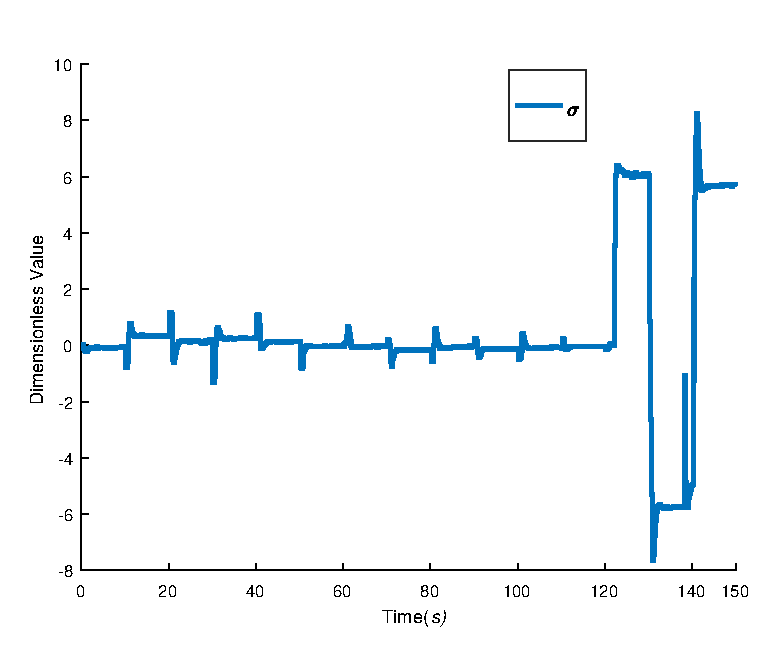
\includegraphics[width=7.0cm,height = 5cm]{figure/chap5/6dof/L1AC/Sigma.pdf}}
  \centerline{(c) }
\end{minipage}
\vfill
\begin{minipage}{0.48\linewidth}
  \centerline{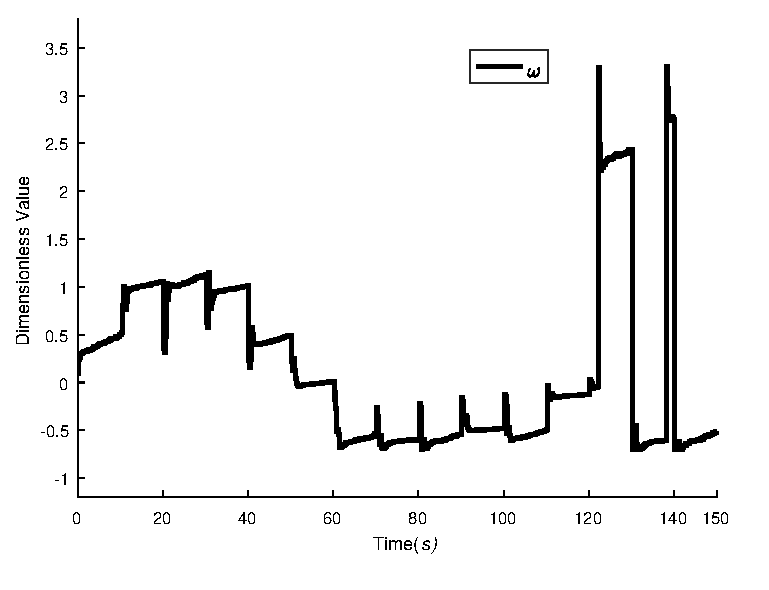
\includegraphics[width=7.0cm,height = 5cm]{figure/chap5/6dof/L1AC/omega.pdf}}
  \centerline{(d) }
\end{minipage}
\label{fig:chap5:F7}
\bicaption[fig:chap5:F7]{存在驱动噪声、测量噪声和干扰时6自由度非线性动态系统的\texorpdfstring {$L_1$}{}自适应控制追踪脉冲输入指令}{存在驱动噪声、测量噪声和干扰时6自由度非线性动态系统的\texorpdfstring {$L_1$}{}自适应控制追踪脉冲输入指令}{Fig.}{ \texorpdfstring {$L_1$}{} adaptive control of the 6 DOF nonlinear dynamic systems for tracking pulse input set-points in the presence of measurement actuator noise and disturbance}
\end{figure}

\begin{figure}[htp]
\centering
\begin{minipage}{0.48\linewidth}
  \centerline{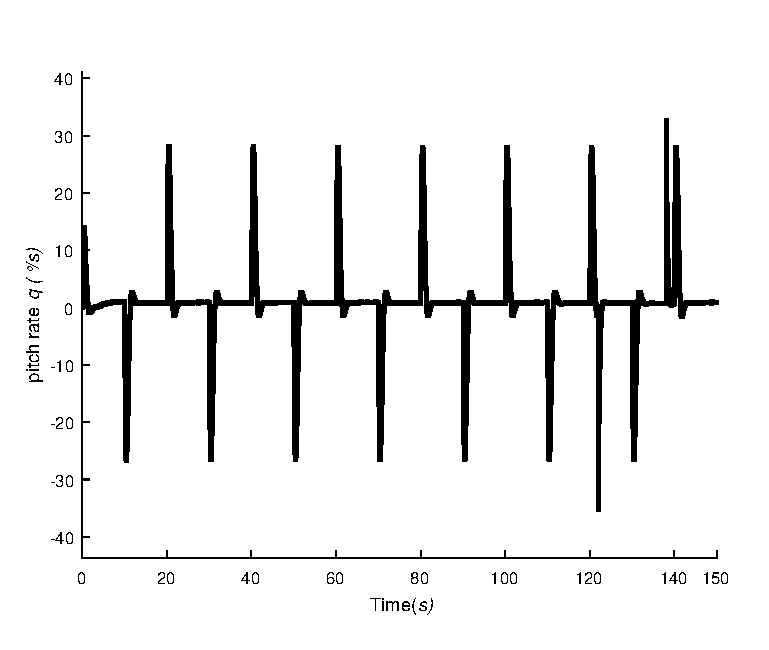
\includegraphics[width=8.0cm,height = 6cm]{figure/chap5/6dof/L1AC/pitch_rate_q.pdf}}
  \centerline{(a) }
\end{minipage}
\vfill
\begin{minipage}{0.48\linewidth}
  \centerline{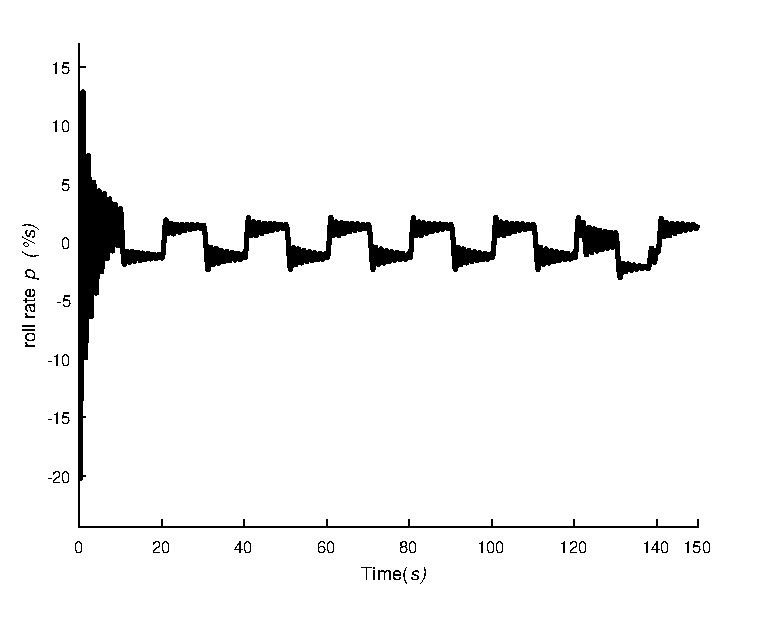
\includegraphics[width=8.0cm,height = 6cm]{figure/chap5/6dof/L1AC/rollrate.pdf}}
  \centerline{(b) }
\end{minipage}
\label{fig:chap5:F8}
\bicaption[fig:chap5:F8]{6自由度非线性动态系统的\texorpdfstring {$L_1$}{}自适应控制追踪脉冲输入指令的俯仰与横滚速率响应}{6自由度非线性动态系统的\texorpdfstring {$L_1$}{}自适应控制追踪脉冲输入指令的俯仰与横滚速率响应}{Fig.}{ Pitch and roll rate response of \texorpdfstring{$L_1$}{} adaptive control of 6 DOF nonlinear vehicle when tracking pulse input set-points}
\end{figure}

%-------------------------------------------------------------------------
\begin{figure}[htp]
\centering
\begin{minipage}{0.9\linewidth}
  \centerline{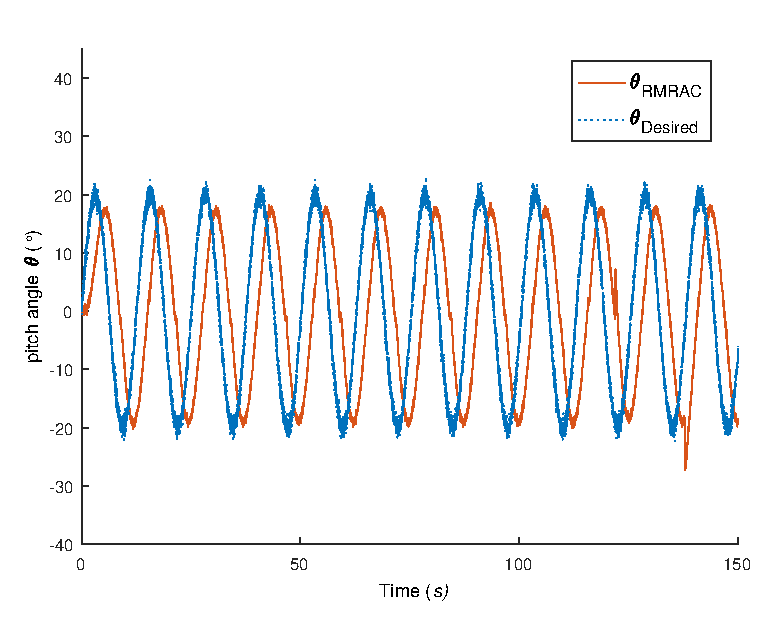
\includegraphics[width=12.0cm,height = 7cm]{figure/chap5/6dof/RMRAC/RMRA_x_sin.pdf}}
  \centerline{(a) }
\end{minipage}
\vfill
\begin{minipage}{0.9\linewidth}
  \centerline{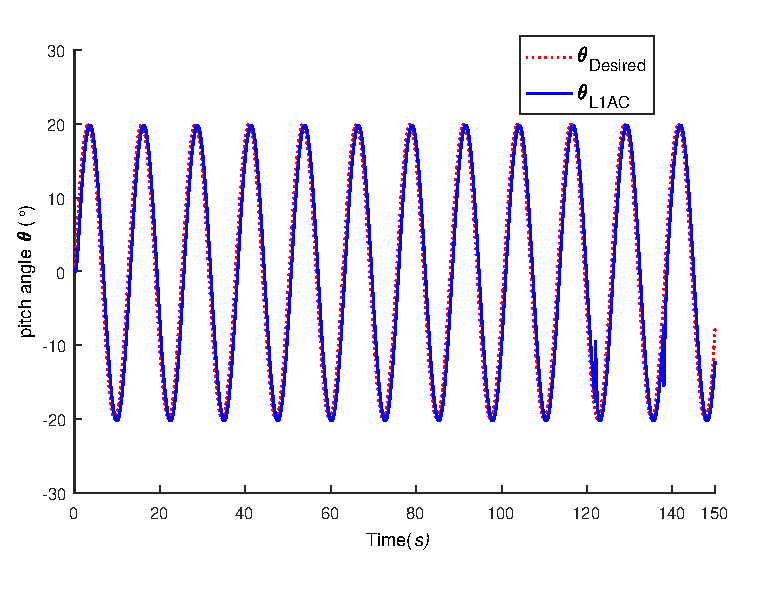
\includegraphics[width=11.0cm,height = 7cm]{figure/chap5/6dof/L1AC/L1AC_x_sin.pdf}}
  \centerline{(b) }
\end{minipage}
\label{fig:chap5:F9}
\bicaption[fig:chap5:F9]{存在驱动噪声、测量噪声和干扰时6自由度非线性动态系统的鲁棒自适应控制与 \texorpdfstring{$L_1$}{} 自适应控制追踪正弦输入指令结果}{存在驱动噪声、测量噪声和干扰时6自由度非线性动态系统的鲁棒自适应控制与 \texorpdfstring{$L_1$}{} 自适应控制追踪正弦输入指令结果}{Fig.}{ Results for robust model reference control and \texorpdfstring{$L_1$}{} adaptive control of the 6 DOF nonlinear dynamic systems for tracking sinusoidal input set-points in the presence of measurement actuator noise and disturbance}
\end{figure}

%------------------------------------------------------------------------

\begin{figure}[H]
\centering
\begin{minipage}{0.9\linewidth}
  \centerline{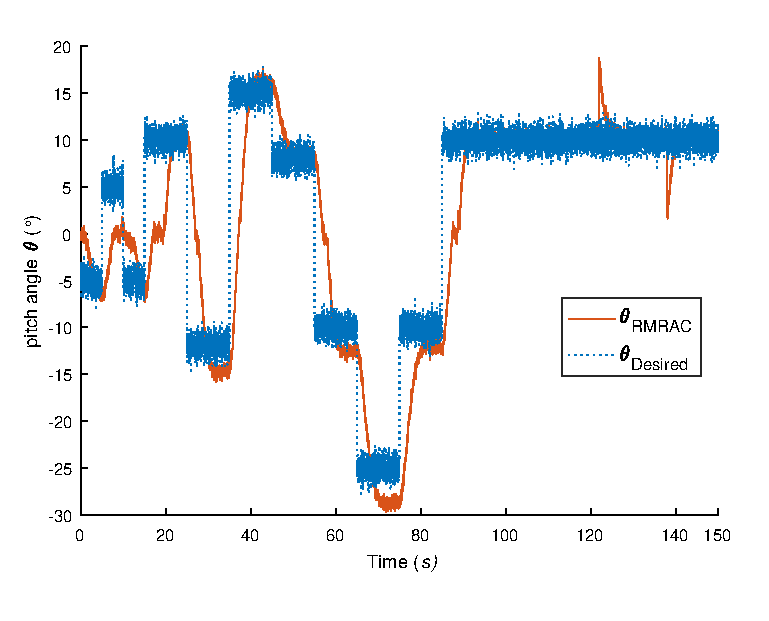
\includegraphics[width=12.0cm,height = 7cm]{figure/chap5/6dof/RMRAC/RMRA_x.pdf}}
  \centerline{(a) }
\end{minipage}
\vfill
\begin{minipage}{0.9\linewidth}
  \centerline{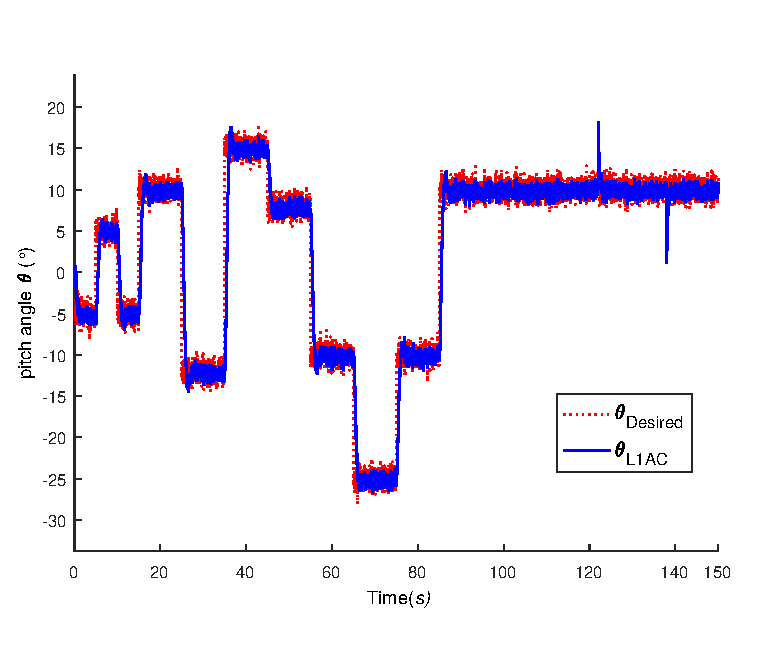
\includegraphics[width=12.0cm,height = 7cm]{figure/chap5/6dof/L1AC/L1AC_x.pdf}}
  \centerline{(b) }
\end{minipage}
\label{fig:chap5:F10}
\bicaption[fig:chap5:F10]{存在驱动噪声、测量噪声和干扰时6自由度非线性动态系统的 \texorpdfstring{$L_1$}{} 自适应控制追踪随意输入指令}{存在驱动噪声、测量噪声和干扰时6自由度非线性动态系统的 \texorpdfstring{$L_1$}{} 自适应控制追踪随意输入指令}{Fig.}{ \texorpdfstring{$L_1$}{} adaptive control of the 6 DOF nonlinear dynamic systems for tracking random input set-points in the presence of measurement actuator noise and disturbance}
\end{figure}


同样,随意设定的期望俯仰角度指令也被输入到鲁棒自适应控制器和$L_1$自适应控制器中,虽然控制器受到噪声和干扰的影响,两种自适应控制器都能表现出良好的鲁棒性和抗扰性。图\ref{fig:chap5:F10}中也进一步说明了$L_1$自适应控制器用于REMUS水下机器人的俯仰角度控制更加具有优越性。


\section{本章小结 }

本章首先系统地分析了水下机器人的非线性和不确定性等系统特性,确定水下机器人模型结构参数估计误差和模型中存在的未建模动态是设计水下机器人控制器需要面对的主要挑战。考虑模型结构不确定性、参数模型不确定性以及非线性,给出了状态模型参考自适应控制方法,该方案可以确保系统可以自适应地应对更多的不确定性。针对状态模型参考自适应控制中的参数漂移和未建模动态问题,使用射影算子理论来确保自适应增益的有界性,进而确保闭环系统的鲁棒性。针对模型参考自适应框架中存在的自适应更新慢,鲁棒性与自适应耦合的问题,提出使用$L_1$自适应控制用以改善水下机器人的俯仰姿态的控制效果。考虑噪声干扰、瞬间扰动的情况下,分别将鲁棒模型参考自适应控制和$L_1$自适应控制用于具有高度非线性与耦合的6自由度REMUS 水下机器人的俯仰自由度的姿态控制,对比水下机器人跟踪随意设定的期望指令的响应结果,确定$L_1$控制的可行性和优越性。
